\documentclass{article}

% Language setting
\usepackage[italian]{babel}

% Set page size and margins
\usepackage[a4paper,top=2cm,bottom=2cm,left=2cm,right=2cm,marginparwidth=1.75cm]{geometry}

% Useful packages
\usepackage{amsmath}
\usepackage{amssymb} 
\usepackage{comment}    %scrivere commenti multirighe
\usepackage{graphicx}
\usepackage{microtype}
\usepackage[colorlinks=true,allcolors=teal]{hyperref}
\usepackage{xcolor}
\usepackage{caption, subcaption}

% set san-serif font for all the document
\renewcommand{\familydefault}{\sfdefault}
% text style to create a code snippet
\definecolor{codegray}{gray}{0.9}
\newcommand{\code}[1]{\colorbox{codegray}{\texttt{#1}}}


% Title
\title{\textbf{Relazione Progetto di Calcolo Numerico}}
\author{Benatti Alice, Manuelli Matteo, Qayyum Shahbaz Ali}
\date{Gennaio 2022}

\begin{document}
\maketitle
\addvspace{1cm}
% Summary
\tableofcontents
\addvspace{2cm}
\hrule
% All content
\begin{comment}
Relazione

1. Riportare e commentare i risultati ottenuti nei punti 2. 3. (e 4.) 
su un immagine del set creato e su altre due immagini in bianco e nero 
(fotografiche/mediche/astronomiche)
2. Riportare delle tabelle con le misure di PSNR e MSE ottenute al 
variare dei parametri (dimensione kernel, valore di sigma, la 
deviazione standard del rumore, il parametro di regolarizzazione). 
3. Calcolare sull’intero set di immagini medie e deviazione standard 
delle metriche per alcuni valori fissati dei parametri.  
4. Analizzare su 2 esecuzioni le proprietà dei metodi numerici 
utilizzati (gradiente coniugato e gradiente) in termini di numero di 
iterazioni, andamento dell’errore, della funzione obiettivo, norma del 
gradiente. 
\end{comment}

\section{Presentazione del problema}
L'obiettivo del progetto è comprendere e mettere in atto metodi per la ricostruizione, o recupero, di 
immagini blurrate, lavorando su problemi test, ovvero abbiamo generato corrotte da un rumore 
Gaussiano applicandolo ad un set di immagini pulite in modo tale da analizzare il problema. 

Inizialmente verrà analizzata l'immagine \code{data.camera()} importata da
\code{skimage}, successivamente verranno analizzate 8 immagini con oggetti geometrici
 di colore uniforme su sfondo nero, realizzate da noi.

Il problema di deblur consiste nella ricostruzione di un immagine a partire da un dato acquisito
 mediante il seguente modello:
\[b=Ax+\eta\]
dove $b$ rappresenta l'immagine corrotta, $x$ l'immagine originale che vogliamo ricostruire, $A$ 
l'operatore che applica il blur Gaussiano ed $\eta$ il rumore additivo con distribuzione Gaussiana di
 media 0 e deviazione standard $\sigma$.

Per svolgere il progetto si farà uso dei moduli \code{numpy}, \code{skimage} e \code{matplotlib}
utilizzando il linguaggio Python.

Affinché risultino chiari i valori a cui andremo a riferirci nella relazione, bisogna tenere ben presente 
il significato di questi due parametri. 

\textbf{PSNR (Peak Signal to Noise Ratio):} Misura la qualità di un immagine ricostruita rispetto all'immagine 
originale, la formula per calcolarlo è la seguente: \[PSNR = log_{10}(\frac{max\;x^\ast}{\sqrt{MSE}})\]

\textbf{MSE (Mean Squared Error):}  Con la sigla ci riferiamo all'errore quadratico medio ed è così ottenuto:
 \[MSE = \sqrt[2]{\frac{\sum_{i=1}^n\sum_{j=1}(x^{\ast}_{ij}-x_{ij})}{nm}}\]

I due valori sono inversamente proposizionali; più è alto il PSNR e basso l'MSE, più l'immagine sarà 
simile all'immagine originale. il PSNR dipende dall'MSE.

\textbf{Deviazione standard:} indica quanto sono distribuiti i dati rispetto alla loro media: 
un valore piccolo indica che i dati sono "ammassati" intorno al valore medio, 
mentre un valore grande indica che i dati sono distribuiti lungo tutto il grafico.

\begin{figure}[H]\centering
	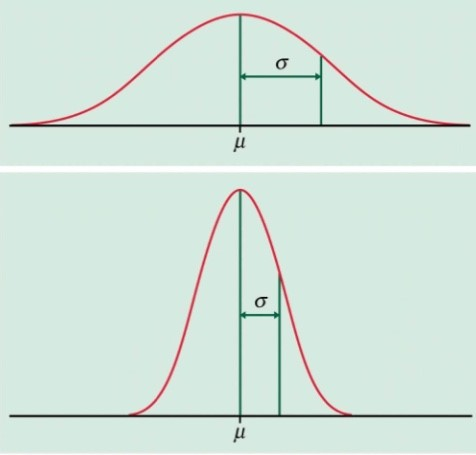
\includegraphics[width=0.3\textwidth]{MANCANTI/deviazione standard.jpg}
	\caption{Distrubuzione valori rispetto ad un valore medio}
\end{figure}
    \subsection{Generazione dataset}
    E' richiesto un set di immagini con le seguenti specifiche: 
\begin{itemize}
    \item 8 Immagini di dimensione $512 \times 512$;
    \item Formato PNG in scala dei grigi;
    \item Devono contenere tra i 2 ed i 6 oggetti geometrici;
    \item Oggetti di colore uniforme su uno sfondo nero.
\end{itemize}


Useremo anche altre due immagini di tipo fotografico/medico/astronomico a scelta trovate su internet.
Quest'ultime saranno importate all'interno del progetto con la libreria \code{skimage}, impostando il flag \verb|as_gray=True| per averle in bianco e nero.

Le immagini selezionate sono le seguenti:
\begin{description}
    \item[Immagine Con Testo] Composizione di prime pagine di giornale con i relativi articoli.
    \item[Immagine Fotografica] Che ritrae il volto di una persona in modo dettagliato e con varie tonalità di grigio.
\end{description}

\begin{figure}
    \centering
    \subfigure
    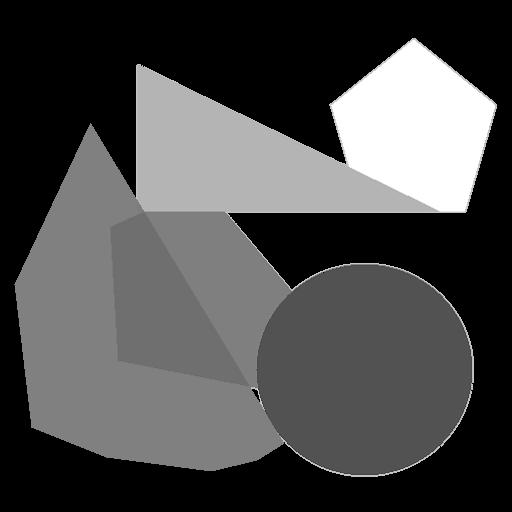
\includegraphics[width=5cm]{img1}\hfil
    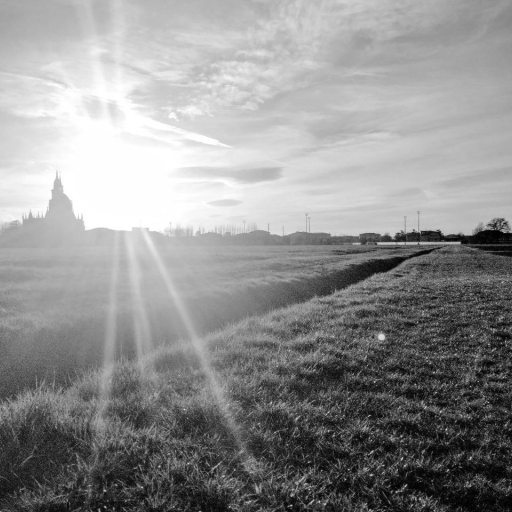
\includegraphics[width=5cm]{paesaggio}
    \caption{Immagine geometrica originale img1.png}
    \label{fig:img1}
    \caption{Immagine fotografica originale paesaggio.png}
    \label{fig:paesaggio}
\end{figure}

    {\color{bblue}\subsection{Generazione Immagini Corrotte}}
\textbf{Obiettivo:}
Degradare le immagini applicando, mediante le funzioni fornite, l'operatore di blur con parametri:
\begin{itemize}
    \item{$\sigma=0.5$ dimensione $5\times 5$}
    \item{$\sigma=1$ dimensione $7\times 7$}
    \item{$\sigma=1.3$ dimensione $9\times 9$}
\end{itemize}
ed aggiungere rumore gaussiano con diversi valori di deviazione standard.

\begin{figure}[H]
    \centering
    \begin{minipage}[h]{\textwidth}
        \centering
        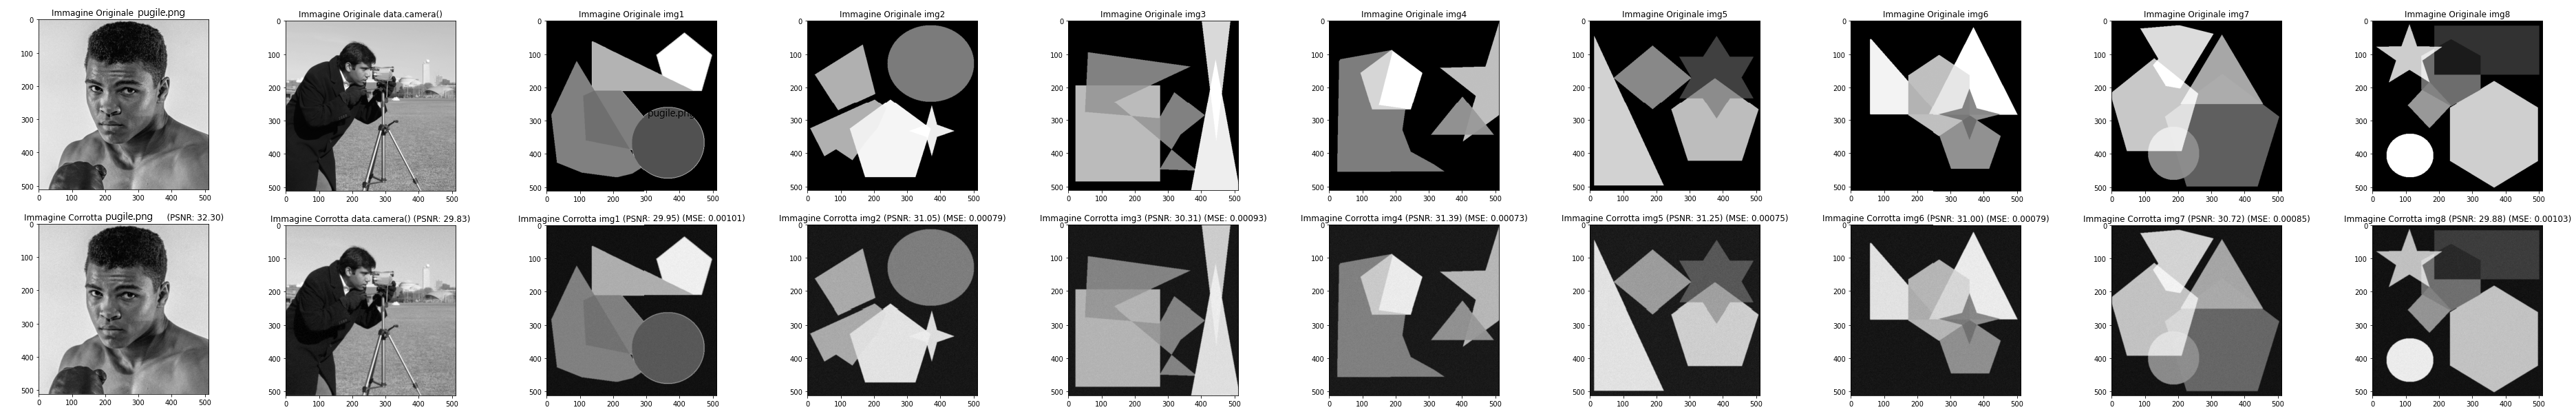
\includegraphics[width=\linewidth]{output/tabCorrotte/imgcorr1.png}\label{fig:imgcorrotte1}
    \end{minipage}
    \begin{minipage}[h]{0.55\textwidth}
        \centering
        \resizebox{1\textwidth}{!}{%
        \begin{tabular}{|l c c c c r|}
            \hline
            \rowcolor{lightbblue}\multicolumn{1}{|c}{\textbf{Nome Img}} & \multicolumn{1}{|c}{\textbf{DimKer}} & \multicolumn{1}{|c}{\textbf{Sigma}} & \multicolumn{1}{|c}{\textbf{Noise Dev}} & \multicolumn{1}{|c}{\textbf{PSNR}} & \multicolumn{1}{|c|}{\textbf{MSE}} \\ \hline
                data.camera() & 5 & 0.5 & 0.02 & 29.8344 & 0.00103886 \\
                pugile.png & 5 & 0.5 & 0.02 & 32.3195 & 0.0005862\\
                img1.png & 5 & 0.5 & 0.02 & 29.9493 & 0.00101175 \\
                img2.png & 5 & 0.5 & 0.02 & 31.0498 & 0.000785276\\
                img3.png & 5 & 0.5 & 0.02 & 30.3053 & 0.000932107\\
                img4.png & 5 & 0.5 & 0.02 & 31.3947 & 0.000725313\\
                img5.png & 5 & 0.5 & 0.02 & 31.2456 & 0.00075065 \\
                img6.png & 5 & 0.5 & 0.02 & 30.9971 & 0.00079486 \\
                img7.png & 5 & 0.5 & 0.02 & 30.7187 & 0.000847478\\
                img8.png & 5 & 0.5 & 0.02 & 29.8802 & 0.00102797 \\ \hline
        \end{tabular}\label{tab:tabcorrotte1}%
        }
    \end{minipage}%
    \begin{minipage}[h]{0.4\textwidth}
        \centering
        \resizebox{0.9\textwidth}{!}{%
        \begin{tabular}{|l r|}
            \hline
            \rowcolor{lightbblue}\multicolumn{2}{|c|}{\textbf{Medie calcolate}} \\ \hline
            Media PSNR           & 30.772611701896455           \\
            Media MSE            & 0.0008494089846671857        \\
            Dev. Std. PSNR       & 0.7547454045875164           \\
            Dev. Std. MSE        & 0.0001420353322461252       \\ \hline
            \end{tabular}
        }
    \end{minipage}
    \captionlistentry[table]{Table corrotte}
    \captionsetup{labelformat=andtable}
    \caption{Immagini corrotte con $\sigma = 0.5$ dimensione $5 \times 5$ e noise = 0.02}
\end{figure}

\begin{figure}[H]
    \centering
    \begin{minipage}[h]{\textwidth}
        \centering
        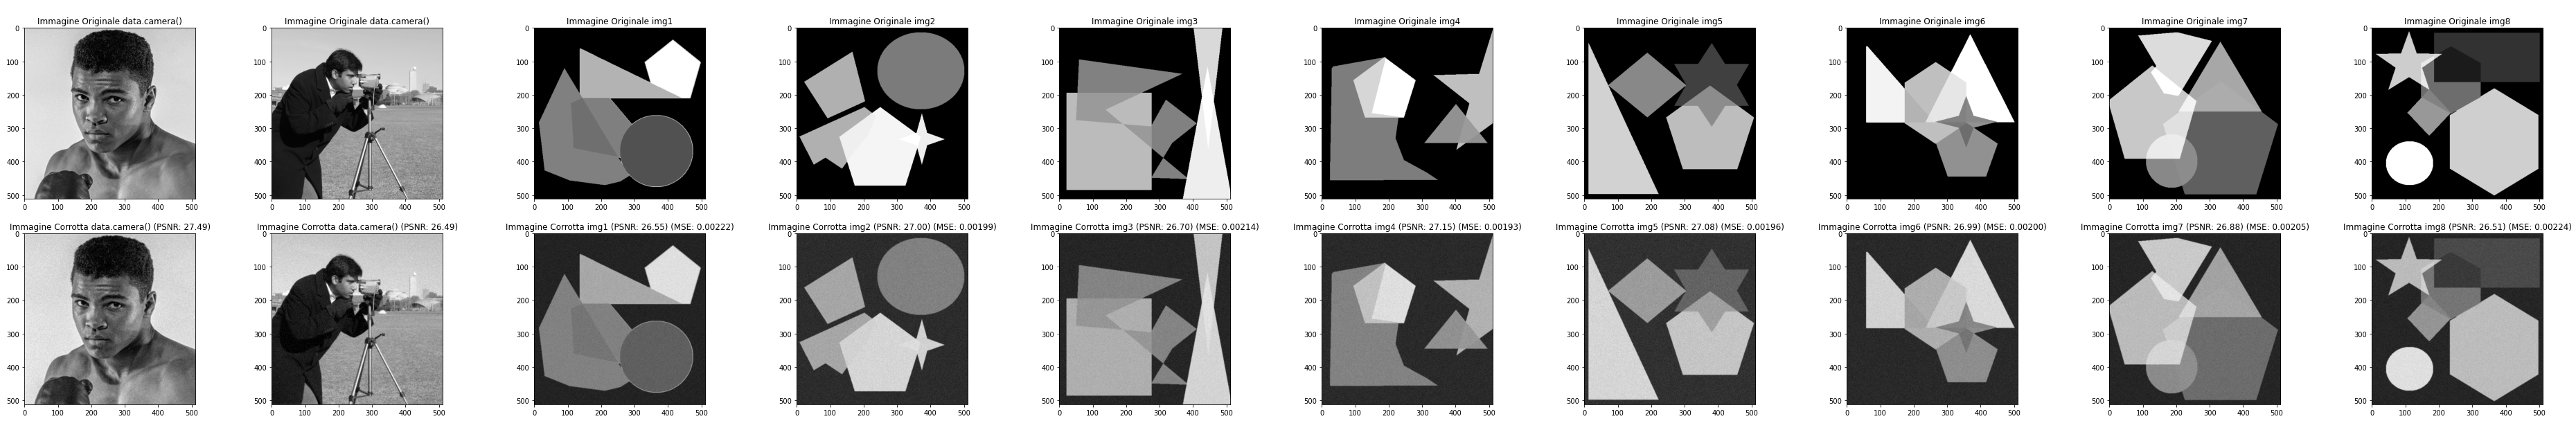
\includegraphics[width=\linewidth]{output/tabCorrotte/imgcorr2.png}\label{fig:imgcorrotte2}
    \end{minipage}
    \begin{minipage}[h]{0.55\textwidth}
        \centering
        \resizebox{1\textwidth}{!}{%
        \begin{tabular}{|l c c c c r|}
            \hline
            \rowcolor{lightbblue}\multicolumn{1}{|c}{\textbf{Nome Img}} & \multicolumn{1}{|c}{\textbf{DimKer}} & \multicolumn{1}{|c}{\textbf{Sigma}} & \multicolumn{1}{|c}{\textbf{Noise Dev}} & \multicolumn{1}{|c}{\textbf{PSNR}} & \multicolumn{1}{|c|}{\textbf{MSE}} \\ \hline
                data.camera() & 5 & 0.5 & 0.04 & 26.5112 & 0.00223297 \\
                pugile.png & 5 & 0.5 & 0.04 & 27.4667 & 0.0017919 \\
                img1.png & 5 & 0.5 & 0.04 & 26.5452 & 0.00221553 \\
                img2.png & 5 & 0.5 & 0.04 & 27.0007 & 0.00199492 \\
                img3.png & 5 & 0.5 & 0.04 & 26.6982 & 0.00213887 \\
                img4.png & 5 & 0.5 & 0.04 & 27.1549 & 0.00192537 \\
                img5.png & 5 & 0.5 & 0.04 & 27.0846 & 0.00195677 \\
                img6.png & 5 & 0.5 & 0.04 & 26.9876 & 0.00200098 \\
                img7.png & 5 & 0.5 & 0.04 & 26.8806 & 0.00205086 \\
                img8.png & 5 & 0.5 & 0.04 & 26.5063 & 0.00223545 \\ \hline
            \end{tabular}\label{tab:tabcorrotte2}%
        }   
        \end{minipage}%
    \begin{minipage}[h]{0.4\textwidth}
        \centering
        \resizebox{0.9\textwidth}{!}{%
        \begin{tabular}{|l r|}
            \hline
            \rowcolor{lightbblue}\multicolumn{2}{|c|}{\textbf{Medie calcolate}} \\ \hline
            Media PSNR           & 26.891734569652385           \\
            Media MSE            & 0.002050504949458885        \\
            Dev. Std. PSNR       & 0.3007954092260605           \\
            Dev. Std. MSE        & 0.00014057036112999103       \\ \hline
            \end{tabular}
        }
    \end{minipage}
    \captionlistentry[table]{Table corrotte}
    \captionsetup{labelformat=andtable}
    \caption{Immagini corrotte con $\sigma = 0.5$ dimensione $5 \times 5$ e noise = 0.04}
\end{figure}

\begin{figure}[H]
    \centering
    \begin{minipage}[h]{\textwidth}
        \centering
        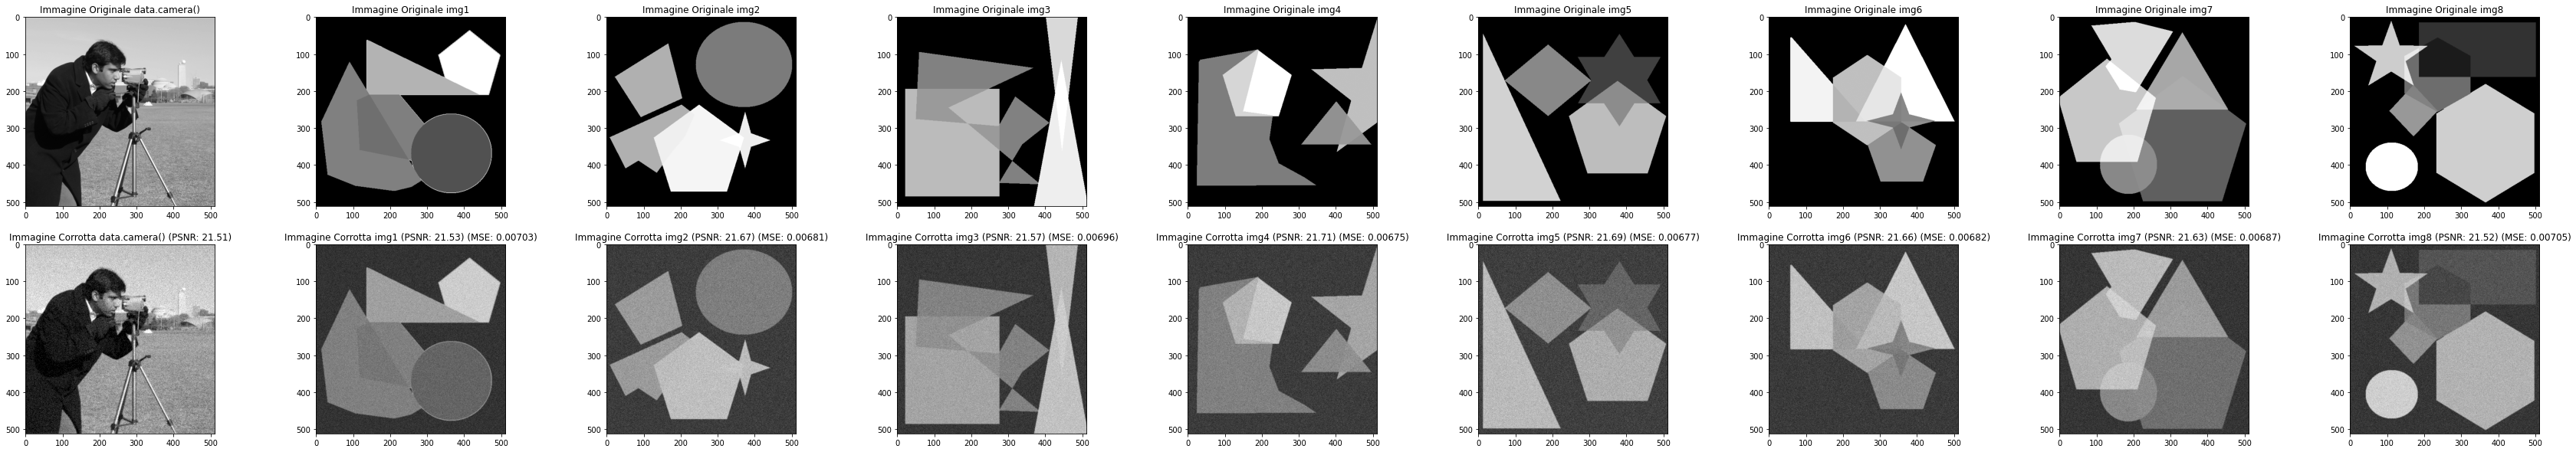
\includegraphics[width=\linewidth]{output/tabCorrotte/imgcorr3.png}\label{fig:imgcorrotte3}
    \end{minipage}
    \begin{minipage}[h]{0.55\textwidth}
        \centering
        \resizebox{1\textwidth}{!}{%
        \begin{tabular}{|l c c c c r|}
            \hline
            \rowcolor{lightbblue}\multicolumn{1}{|c}{\textbf{Nome Img}} & \multicolumn{1}{|c}{\textbf{DimKer}} & \multicolumn{1}{|c}{\textbf{Sigma}} & \multicolumn{1}{|c}{\textbf{Noise Dev}} & \multicolumn{1}{|c}{\textbf{PSNR}} & \multicolumn{1}{|c|}{\textbf{MSE}} \\ \hline
                data.camera() & 5 & 0.5 & 0.08 &  21.5325 &  0.00702666 \\ 
                pugile.png & 5 & 0.5 & 0.08 & 21.7986 & 0.0066091\\ 
                img1.png & 5 & 0.5 & 0.08 & 21.5332 & 0.00702558 \\
                img2.png & 5 & 0.5 & 0.08 & 21.6702 & 0.00680731 \\
                img3.png & 5 & 0.5 & 0.08 & 21.5736 & 0.00696048 \\
                img4.png & 5 & 0.5 & 0.08 & 21.7089 & 0.00674704 \\
                img5.png & 5 & 0.5 & 0.08 & 21.6929 & 0.00677191 \\
                img6.png & 5 & 0.5 & 0.08 & 21.6626 & 0.00681931 \\
                img7.png & 5 & 0.5 & 0.08 & 21.633 & 0.00686601 \\
                img8.png & 5 & 0.5 & 0.08 & 21.519 & 0.00704858 \\\hline
            \end{tabular}\label{tab:tabcorrotte3}%
        }   
        \end{minipage}%
    \begin{minipage}[h]{0.4\textwidth}
        \centering
        \resizebox{0.9\textwidth}{!}{%
        \begin{tabular}{|l r|}
            \hline
            \rowcolor{lightbblue}\multicolumn{2}{|c|}{\textbf{Medie calcolate}} \\ \hline
            Media PSNR           & 21.656429313389726           \\
            Media MSE            & 0.00683046240248098       \\
            Dev. Std. PSNR       & 0.08995967536472305           \\
            Dev. Std. MSE        & 0.00014118437500020744      \\ \hline
            \end{tabular}
        }
    \end{minipage}
    \captionlistentry[table]{Table corrotte}
    \captionsetup{labelformat=andtable}
    \caption{Immagini corrotte con $\sigma = 0.5$ dimensione $5 \times 5$ e noise = 0.08}
\end{figure}

\begin{figure}[H]
    \centering
    \begin{minipage}[h]{\textwidth}
        \centering
        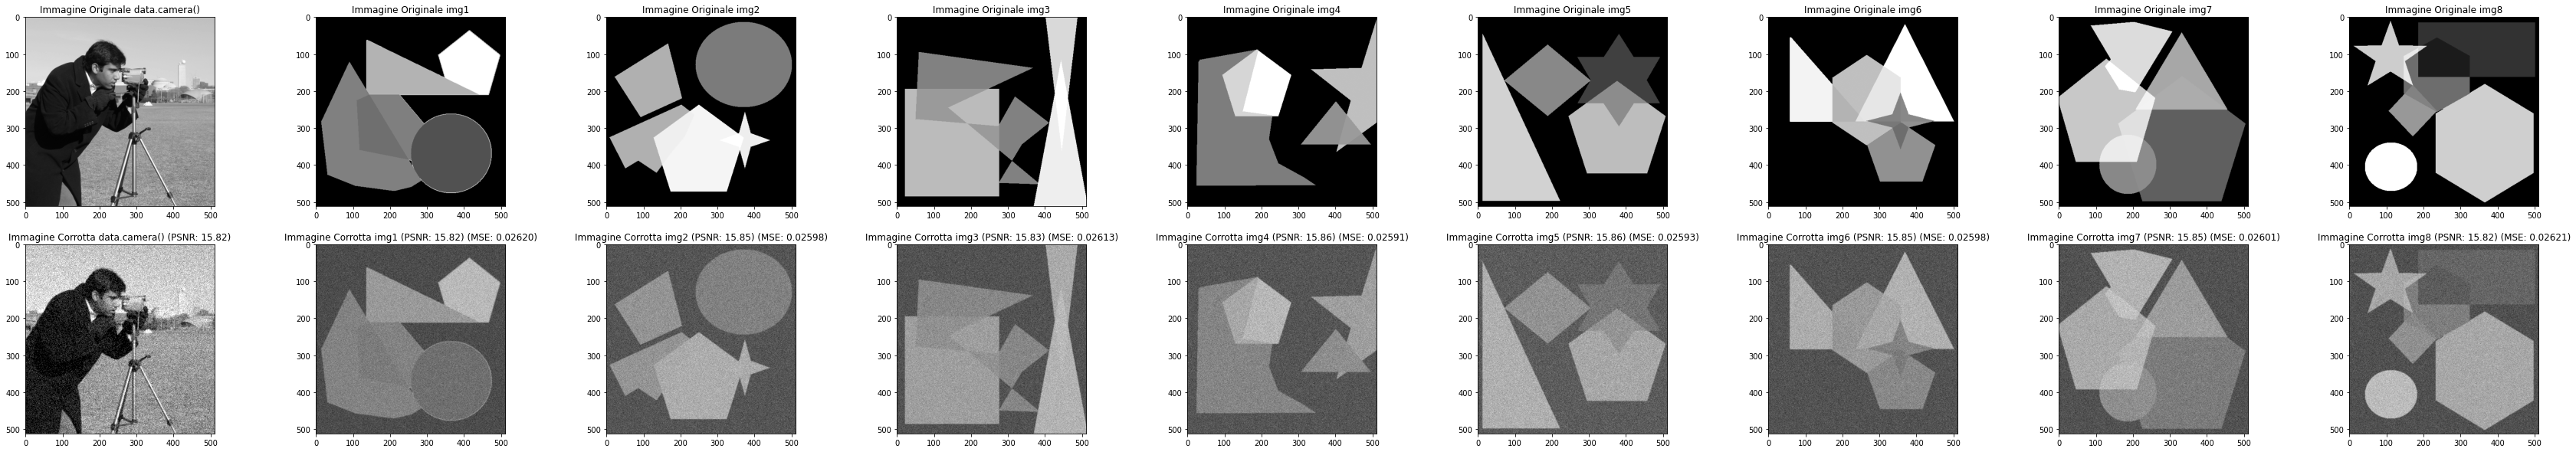
\includegraphics[width=\linewidth]{output/tabCorrotte/imgcorr4.png}\label{fig:imgcorrotte4}
    \end{minipage}
    \begin{minipage}[h]{0.55\textwidth}
        \centering
        \resizebox{1\textwidth}{!}{%
        \begin{tabular}{|l c c c c r|}
            \hline
            \rowcolor{lightbblue}\multicolumn{1}{|c}{\textbf{Nome Img}} & \multicolumn{1}{|c}{\textbf{DimKer}} & \multicolumn{1}{|c}{\textbf{Sigma}} & \multicolumn{1}{|c}{\textbf{Noise Dev}} & \multicolumn{1}{|c}{\textbf{PSNR}} & \multicolumn{1}{|c|}{\textbf{MSE}} \\ \hline
                data.camera() & 5 & 0.5 & 0.16 & 15.7869 & 0.0263819 \\
                pugile.png & 5 & 0.5 & 0.16 & 15.89 & 0.0257632 \\
                img1.png & 5 & 0.5 & 0.16 & 15.8162 & 0.0262048 \\
                img2.png & 5 & 0.5 & 0.16 & 15.8543 & 0.025976 \\
                img3.png & 5 & 0.5 & 0.16 & 15.8278 & 0.0261347 \\
                img4.png & 5 & 0.5 & 0.16 & 15.8649 & 0.0259124 \\
                img5.png & 5 & 0.5 & 0.16 & 15.8618 & 0.0259313 \\
                img6.png & 5 & 0.5 & 0.16 & 15.8537 & 0.0259797 \\
                img7.png & 5 & 0.5 & 0.16 & 15.849 & 0.0260077 \\
                img8.png & 5 & 0.5 & 0.16 & 15.8161 & 0.0262051 \\ \hline
            \end{tabular}\label{tab:tabcorrotte4}%
        }   
        \end{minipage}%
    \begin{minipage}[h]{0.4\textwidth}
        \centering
        \resizebox{0.9\textwidth}{!}{%
        \begin{tabular}{|l r|}
            \hline
            \rowcolor{lightbblue}\multicolumn{2}{|c|}{\textbf{Medie calcolate}} \\ \hline
            Media PSNR           & 15.821291629768288           \\
            Media MSE            & 0.026174436676272776        \\
            Dev. Std. PSNR       & 0.02377710929356369          \\
            Dev. Std. MSE        & 0.00014322778885193189       \\ \hline
            \end{tabular}
        }
    \end{minipage}
    \captionlistentry[table]{Table corrotte}
    \captionsetup{labelformat=andtable}
    \caption{Immagini corrotte con $\sigma = 0.5$ dimensione $5 \times 5$ e noise = 0.16}
\end{figure}

\begin{figure}[H]
    \centering
    \begin{minipage}[h]{\textwidth}
        \centering
        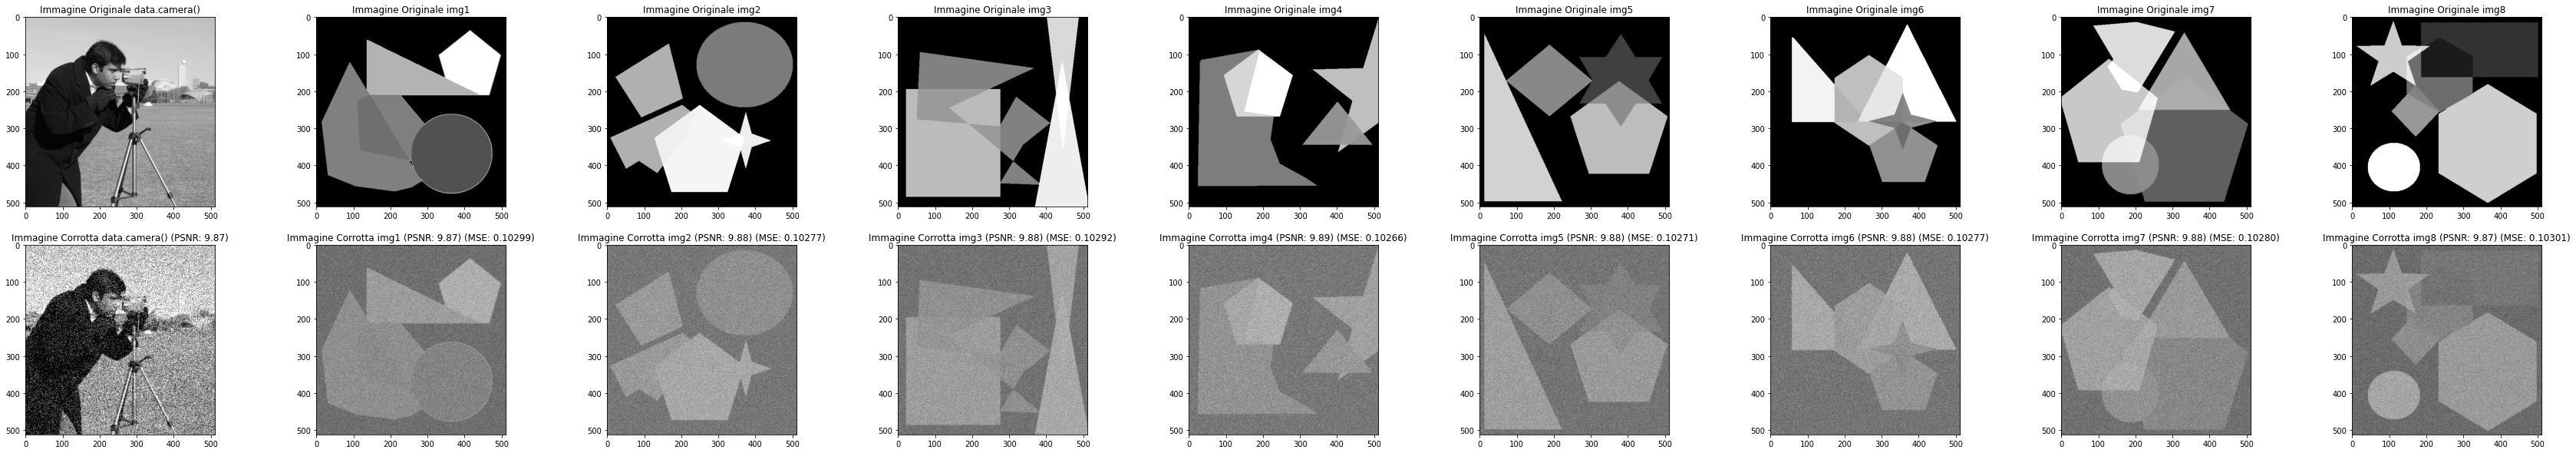
\includegraphics[width=\linewidth]{output/tabCorrotte/imgcorr5.png}\label{fig:imgcorrotte5}
    \end{minipage}
    \begin{minipage}[h]{0.55\textwidth}
        \centering
        \resizebox{1\textwidth}{!}{%
        \begin{tabular}{|l c c c c r|}
            \hline
            \rowcolor{lightbblue}\multicolumn{1}{|c}{\textbf{Nome Img}} & \multicolumn{1}{|c}{\textbf{DimKer}} & \multicolumn{1}{|c}{\textbf{Sigma}} & \multicolumn{1}{|c}{\textbf{Noise Dev}} & \multicolumn{1}{|c}{\textbf{PSNR}} & \multicolumn{1}{|c|}{\textbf{MSE}} \\ \hline
                data.camera() & 5 & 0.5 & 0.32 & 9.90122 & 0.102301 \\
                pugile.png & 5 & 0.5 & 0.32 & 9.89115 & 0.102538 \\
                img1.png & 5 & 0.5 & 0.32 & 9.8721 & 0.102989 \\                 
                img2.png & 5 & 0.5 & 0.32 & 9.88127 & 0.102772 \\ 
                img3.png & 5 & 0.5 & 0.32 & 9.87516 & 0.102916 \\
                img4.png & 5 & 0.5 & 0.32 & 9.8862 & 0.102655 \\                 
                img5.png & 5 & 0.5 & 0.32 & 9.88405 & 0.102706 \\ 
                img6.png & 5 & 0.5 & 0.32 & 9.88154 & 0.102765 \\
                img7.png & 5 & 0.5 & 0.32 & 9.88 & 0.102802 \\              
                img8.png & 5 & 0.5 & 0.32 & 9.87102 & 0.103014 \\  \hline
            \end{tabular}\label{tab:tabcorrotte5}%
        }     
        \end{minipage}%
    \begin{minipage}[h]{0.4\textwidth}
        \centering
        \resizebox{0.9\textwidth}{!}{%
        \begin{tabular}{|l r|}
            \hline
            \rowcolor{lightbblue}\multicolumn{2}{|c|}{\textbf{Medie calcolate}} \\ \hline
            Media PSNR           & 9.908921219921675         \\
            Media MSE            & 0.10211940428183572      \\
            Dev. Std. PSNR       & 0.005854966950232008        \\
            Dev. Std. MSE        & 0.00013766495799610393     \\ \hline
            \end{tabular}
        }
    \end{minipage}
    \captionlistentry[table]{Table corrotte}
    \captionsetup{labelformat=andtable}
    \caption{Immagini corrotte con $\sigma = 0.5$ dimensione $5 \times 5$ e noise = 0.32}
\end{figure}

\begin{figure}[H]
    \centering
    \begin{minipage}[h]{\textwidth}
        \centering
        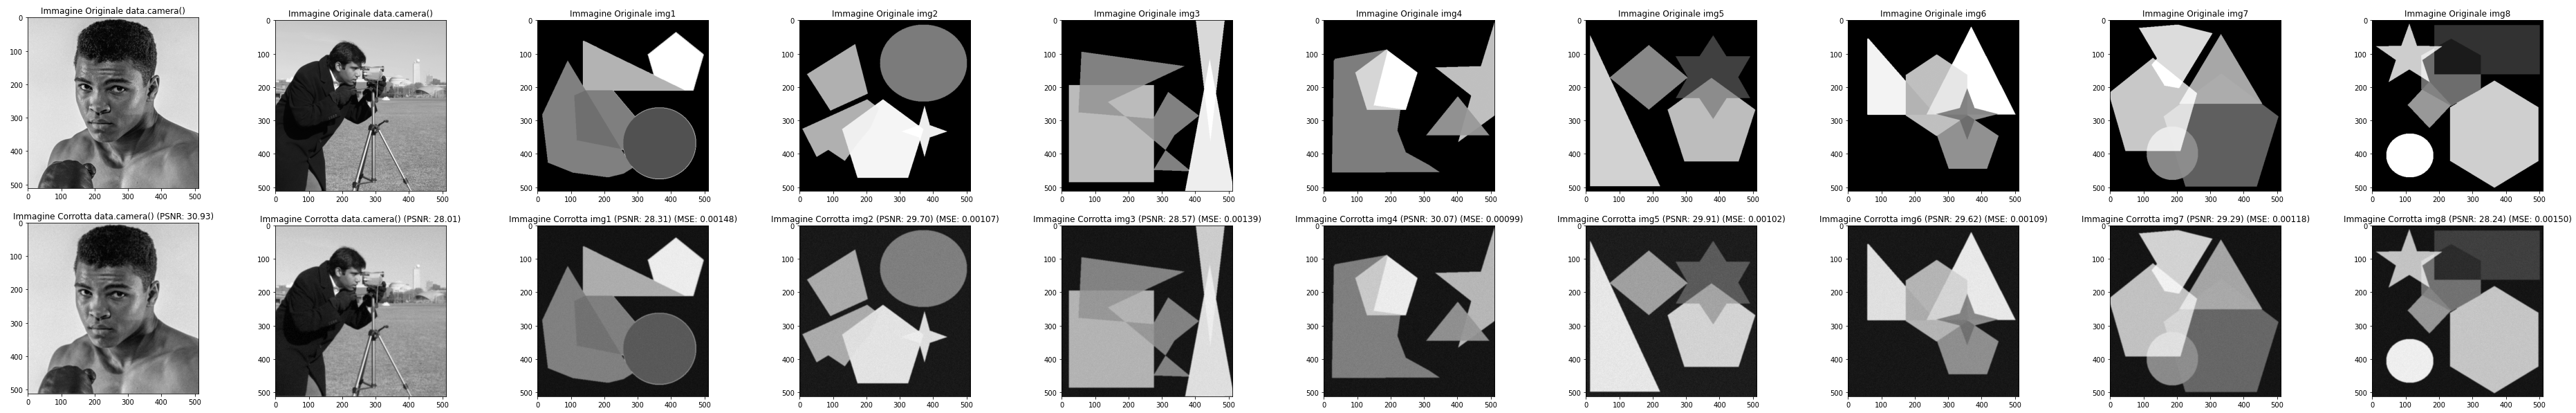
\includegraphics[width=\linewidth]{output/tabCorrotte/imgcorr6.png}\label{fig:imgcorrotte6}
    \end{minipage}
    \begin{minipage}[h]{0.55\textwidth}
        \centering
        \resizebox{1\textwidth}{!}{%
        \begin{tabular}{|l c c c c r|}
            \hline
            \rowcolor{lightbblue}\multicolumn{1}{|c}{\textbf{Nome Img}} & \multicolumn{1}{|c}{\textbf{DimKer}} & \multicolumn{1}{|c}{\textbf{Sigma}} & \multicolumn{1}{|c}{\textbf{Noise Dev}} & \multicolumn{1}{|c}{\textbf{PSNR}} & \multicolumn{1}{|c|}{\textbf{MSE}} \\ \hline
                data.camera() & 7 & 1 & 0.02 & 27.9965 & 0.00158617 \\
                pugile.png & 7 & 1 & 0.02 & 30.9284 & 0.000807527 \\
                img1.png & 7 & 1 & 0.02 & 28.3054 & 0.00147726 \\
                img2.png & 7 & 1 & 0.02 & 29.7038 & 0.00107057 \\
                img3.png & 7 & 1 & 0.02 & 28.5689 & 0.00139029 \\
                img4.png & 7 & 1 & 0.02 & 30.0656 & 0.000985011 \\
                img5.png & 7 & 1 & 0.02 & 29.9064 & 0.0010218 \\                 
                img6.png & 7 & 1 & 0.02 & 29.6228 & 0.00109074 \\ 
                img7.png & 7 & 1 & 0.02 & 29.2918 & 0.00117711 \\
                img8.png & 7 & 1 & 0.02 & 28.2434 & 0.00149851 \\ \hline
            \end{tabular}\label{tab:tabcorrotte6}%
        }   
        \end{minipage}%
    \begin{minipage}[h]{0.4\textwidth}
        \centering
        \resizebox{0.9\textwidth}{!}{%
        \begin{tabular}{|l r|}
            \hline
            \rowcolor{lightbblue}\multicolumn{2}{|c|}{\textbf{Medie calcolate}} \\ \hline
            Media PSNR           & 29.2560497491376        \\
            Media MSE            & 0.0012124124340562978       \\
            Dev. Std. PSNR       & 0.903380822617657        \\
            Dev. Std. MSE        & 0.00024716496411134373      \\ \hline
            \end{tabular}
        }
    \end{minipage}
    \captionlistentry[table]{Table corrotte}
    \captionsetup{labelformat=andtable}
    \caption{Immagini corrotte con $\sigma = 1$ dimensione $7 \times 7$ e noise = 0.02}
\end{figure}

\begin{figure}[H]
    \centering
    \begin{minipage}[h]{\textwidth}
        \centering
        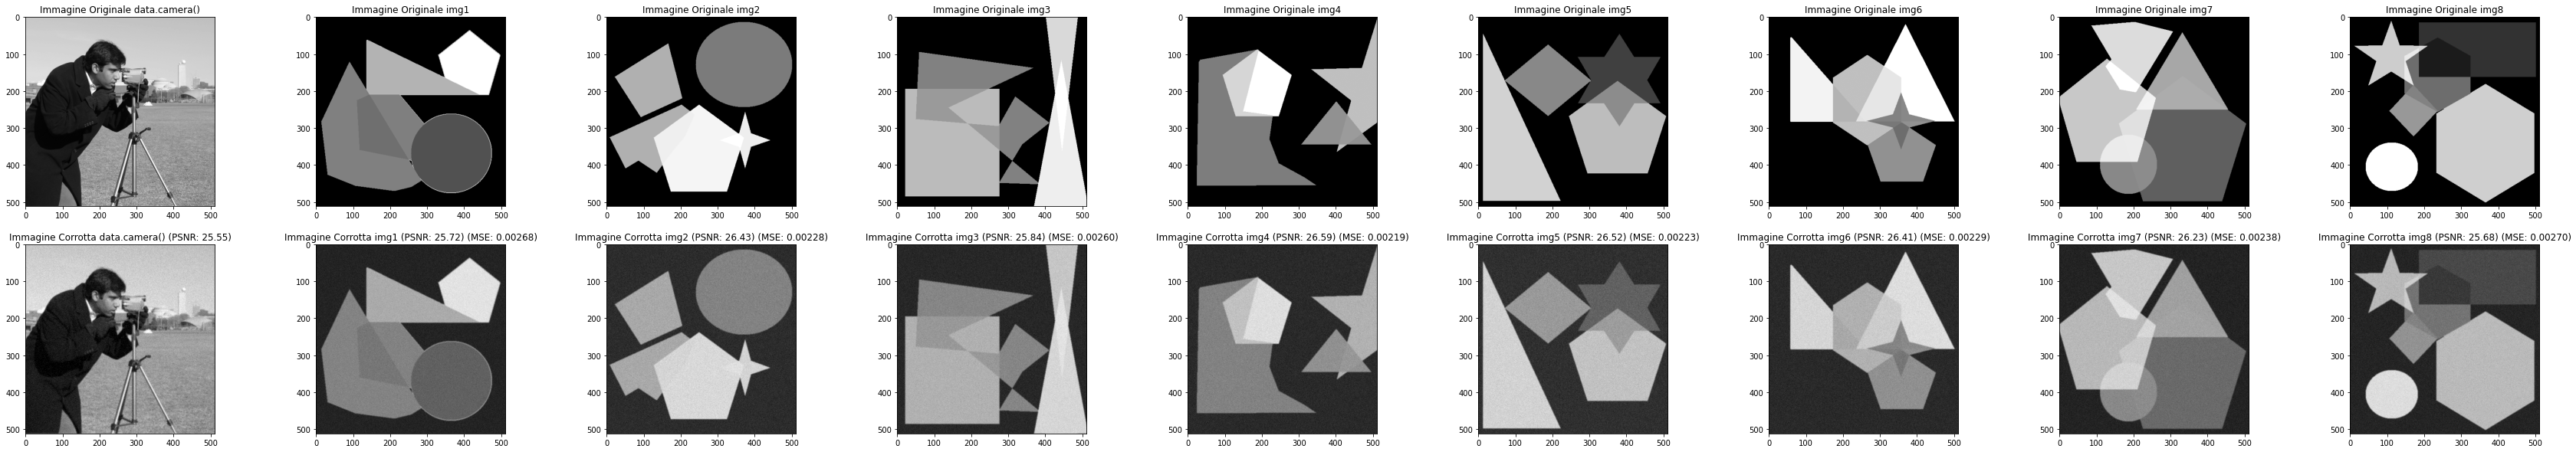
\includegraphics[width=\linewidth]{output/tabCorrotte/imgcorr7.png}\label{fig:imgcorrotte7}
    \end{minipage}
    \begin{minipage}[h]{0.55\textwidth}
        \centering
        \resizebox{1\textwidth}{!}{%
        \begin{tabular}{|l c c c c r|}
            \hline
            \rowcolor{lightbblue}\multicolumn{1}{|c}{\textbf{Nome Img}} & \multicolumn{1}{|c}{\textbf{DimKer}} & \multicolumn{1}{|c}{\textbf{Sigma}} & \multicolumn{1}{|c}{\textbf{Noise Dev}} & \multicolumn{1}{|c}{\textbf{PSNR}} & \multicolumn{1}{|c|}{\textbf{MSE}} \\ \hline
                data.camera() & 7 & 1 & 0.04 & 25.5438 & 0.00279009 \\
                pugile.png & 7 & 1 & 0.04 & 26.9696 & 0.00200928 \\
                img1.png & 7 & 1 & 0.04 & 25.7196 & 0.00267942 \\
                img2.png & 7 & 1 & 0.04 & 26.4282 & 0.00227604 \\
                img3.png & 7 & 1 & 0.04 & 25.8439 & 0.00260379 \\
                img4.png & 7 & 1 & 0.04 & 26.5898 & 0.0021929 \\                
                img5.png & 7 & 1 & 0.04 & 26.5209 & 0.00222797 \\ 
                img6.png & 7 & 1 & 0.04 & 26.4067 & 0.00228732 \\
                img7.png & 7 & 1 & 0.04 & 26.2277 & 0.00238357 \\
                img8.png & 7 & 1 & 0.04 & 25.6828 & 0.00270224 \\ \hline
            \end{tabular}\label{tab:tabcorrotte7}%    
        }   
        \end{minipage}%
    \begin{minipage}[h]{0.4\textwidth}
        \centering
        \resizebox{0.9\textwidth}{!}{%
        \begin{tabular}{|l r|}
            \hline
            \rowcolor{lightbblue}\multicolumn{2}{|c|}{\textbf{Medie calcolate}} \\ \hline
            Media PSNR           & 26.195844232338864         \\
            Media MSE            & 0.0024139860627763257       \\
            Dev. Std. PSNR       & 0.4492018368928465       \\
            Dev. Std. MSE        & 0.0002491578891141964     \\ \hline
            \end{tabular}
        }
    \end{minipage}
    \captionlistentry[table]{Table corrotte}
    \captionsetup{labelformat=andtable}
    \caption{Immagini corrotte con $\sigma = 1$ dimensione $7 \times 7$ e noise = 0.04}
\end{figure}

\begin{figure}[H]
    \centering
    \begin{minipage}[h]{\textwidth}
        \centering
        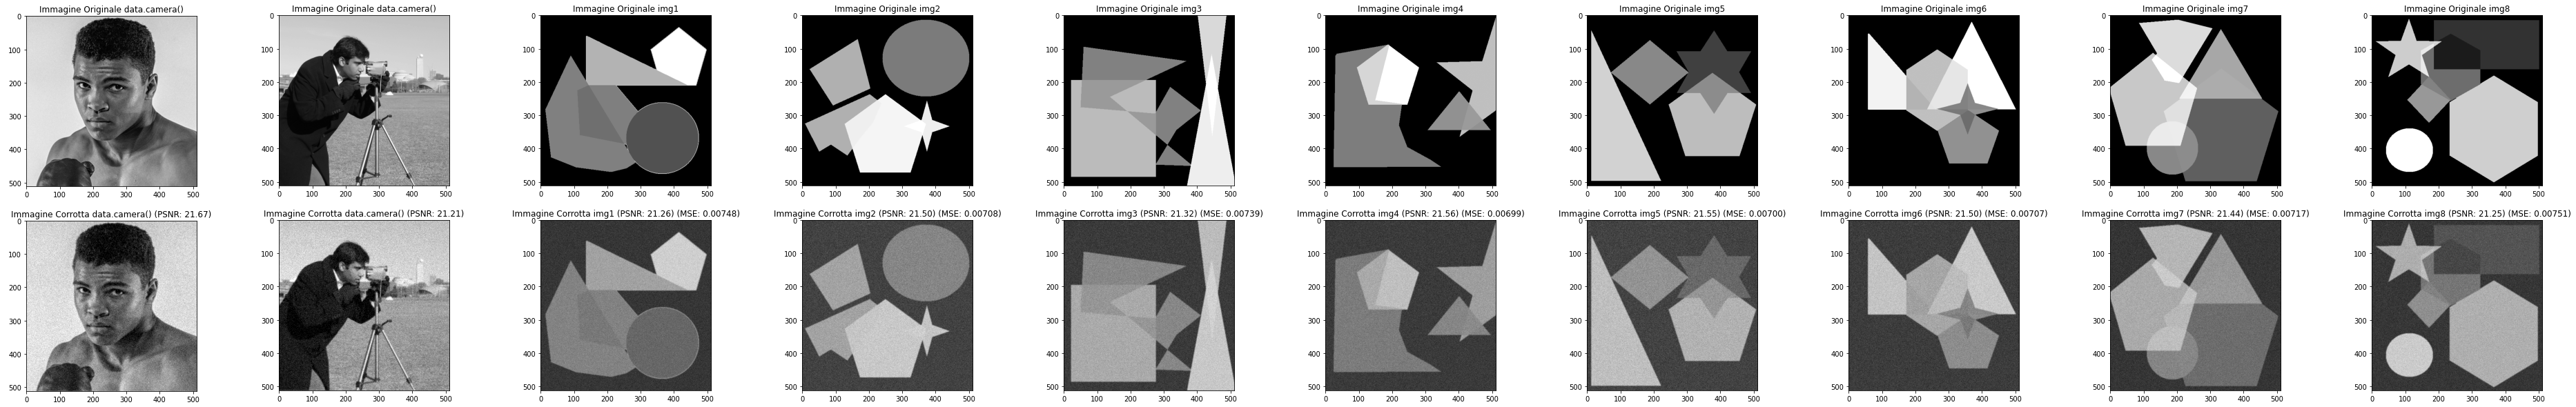
\includegraphics[width=\linewidth]{output/tabCorrotte/imgcorr8.png}\label{fig:imgcorrotte7x70.08}
    \end{minipage}
    \begin{minipage}[h]{0.55\textwidth}
        \centering
        \resizebox{1\textwidth}{!}{%
        \begin{tabular}{|l c c c c r|}
            \hline
            \rowcolor{lightbblue}\multicolumn{1}{|c}{\textbf{Nome Img}} & \multicolumn{1}{|c}{\textbf{DimKer}} & \multicolumn{1}{|c}{\textbf{Sigma}} & \multicolumn{1}{|c}{\textbf{Noise Dev}} & \multicolumn{1}{|c}{\textbf{PSNR}} & \multicolumn{1}{|c|}{\textbf{MSE}} \\ \hline
                data.camera() & 7 & 1 & 0.08 & 21.2232 &  0.0075453 \\
                pugile.png & 7 & 1 & 0.08 & 21.6733 & 0.00680245 \\ 
                img1.png & 7 & 1 & 0.08 & 21.2586 & 0.00748406 \\
                img2.png & 7 & 1 & 0.08 & 21.5025 & 0.00707543 \\
                img3.png & 7 & 1 & 0.08 & 21.3156 & 0.0073866 \\                 
                img4.png & 7 & 1 & 0.08 & 21.5582 & 0.00698523 \\
                img5.png & 7 & 1 & 0.08 & 21.5463 & 0.00700433 \\
                img6.png & 7 & 1 & 0.08 & 21.5043 & 0.00707252 \\
                img7.png & 7 & 1 & 0.08 & 21.4429 & 0.00717307 \\
                img8.png & 7 & 1 & 0.08 & 21.2464 & 0.00750518 \\\hline
            \end{tabular}\label{tab:tabcorrotte7x70.08}%
        }
        \end{minipage}%
    \begin{minipage}[h]{0.4\textwidth}
        \centering
        \resizebox{0.9\textwidth}{!}{%
        \begin{tabular}{|l r|}
            \hline
            \rowcolor{lightbblue}\multicolumn{2}{|c|}{\textbf{Medie calcolate}} \\ \hline
            Media PSNR           & 21.429621292884747         \\
            Media MSE            & 0.0071992640601343085     \\
            Dev. Std. PSNR       & 0.14744138849178753         \\
            Dev. Std. MSE        & 0.0002443541830272355     \\ \hline
            \end{tabular}
        }
    \end{minipage}
    \captionlistentry[table]{Table corrotte}
    \captionsetup{labelformat=andtable}
    \caption{Immagini corrotte con $\sigma = 1$ dimensione $7 \times 7$ e noise = 0.08}
\end{figure}

\begin{figure}[H]
    \centering
    \begin{minipage}[h]{\textwidth}
        \centering
        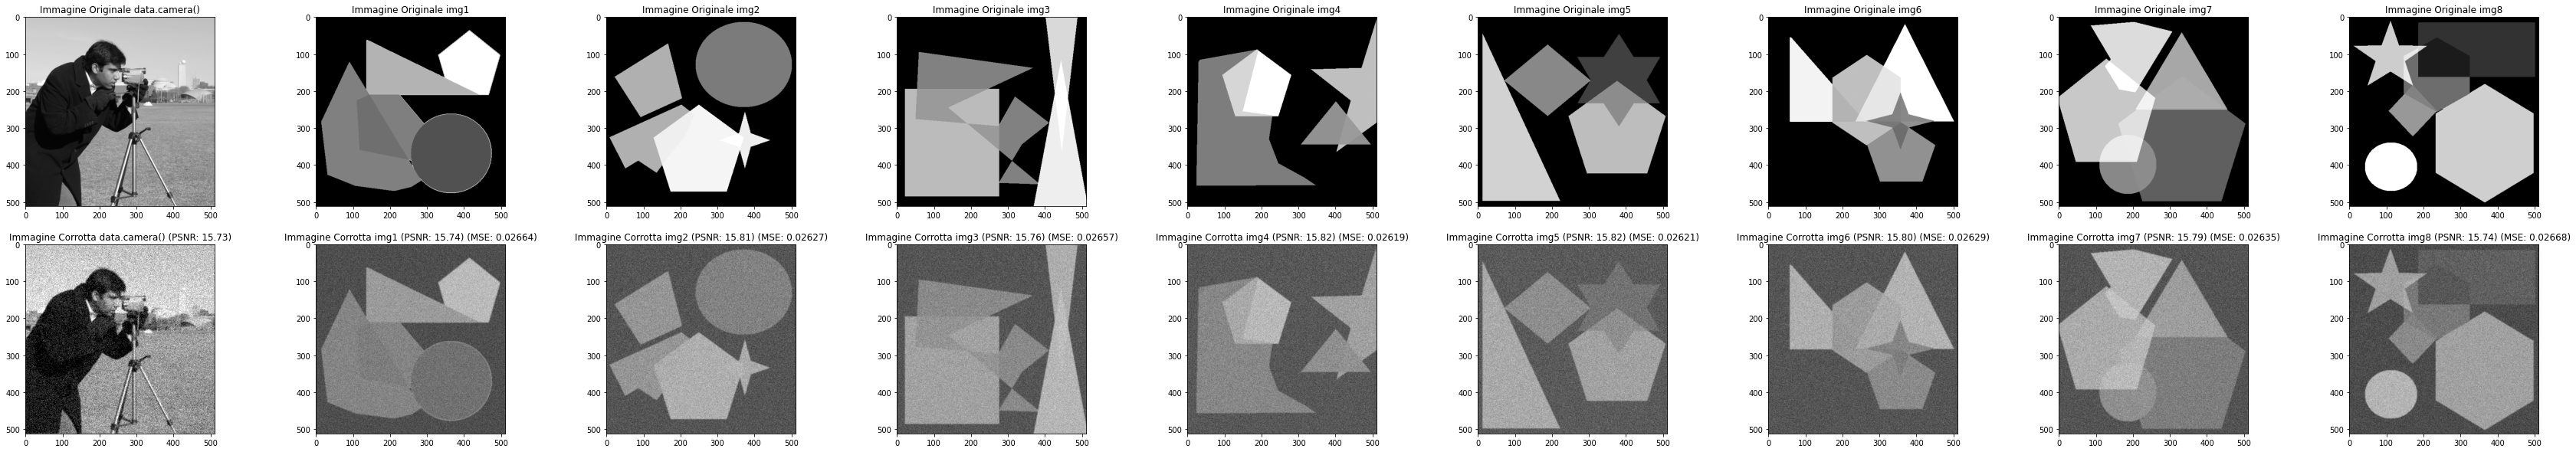
\includegraphics[width=\linewidth]{output/tabCorrotte/imgcorr9.png}\label{fig:imgcorrotte7x70.16}
    \end{minipage}
    \begin{minipage}[h]{0.55\textwidth}
        \centering
        \resizebox{1\textwidth}{!}{%
        \begin{tabular}{|l c c c c r|}
            \hline
            \rowcolor{lightbblue}\multicolumn{1}{|c}{\textbf{Nome Img}} & \multicolumn{1}{|c}{\textbf{DimKer}} & \multicolumn{1}{|c}{\textbf{Sigma}} & \multicolumn{1}{|c}{\textbf{Noise Dev}} & \multicolumn{1}{|c}{\textbf{PSNR}} & \multicolumn{1}{|c|}{\textbf{MSE}} \\ \hline
                data.camera() & 7 & 1 & 0.16 & 15.7309 & 0.0267244 \\
                pugile.png & 7 & 1 & 0.16 & 15.8496 & 0.0260039 \\
                img1.png & 7 & 1 & 0.16 & 15.7444 & 0.0266415 \\
                img2.png & 7 & 1 & 0.16 & 15.8054 & 0.0262698 \\ 
                img3.png & 7 & 1 & 0.16 & 15.7565 & 0.0265673 \\                 
                img4.png & 7 & 1 & 0.16 & 15.8194 & 0.0261856 \\
                img5.png & 7 & 1 & 0.16 & 15.8151 & 0.0262111 \\                 
                img6.png & 7 & 1 & 0.16 & 15.8029 & 0.0262853 \\
                img7.png & 7 & 1 & 0.16 & 15.7926 & 0.0263473 \\                 
                img8.png & 7 & 1 & 0.16 & 15.7385 & 0.0266776 \\\hline
            \end{tabular}\label{tab:tabcorrotte7x70.16}%
        }   
        
        \end{minipage}%
    \begin{minipage}[h]{0.4\textwidth}
        \centering
        \resizebox{0.9\textwidth}{!}{%
        \begin{tabular}{|l r|}
            \hline
            \rowcolor{lightbblue}\multicolumn{2}{|c|}{\textbf{Medie calcolate}} \\ \hline
            Media PSNR           & 15.79693992935469          \\
            Media MSE            & 0.026322419224025406    \\
            Dev. Std. PSNR       & 0.04145677255353015          \\
            Dev. Std. MSE        & 0.00025141610640160646      \\ \hline
            \end{tabular}
        }
    \end{minipage}
    \captionlistentry[table]{Table corrotte}
    \captionsetup{labelformat=andtable}
    \caption{Immagini corrotte con $\sigma = 1$ dimensione $7 \times 7$ e noise = 0.16}
\end{figure}

\begin{figure}[H]
    \centering
    \begin{minipage}[h]{\textwidth}
        \centering
        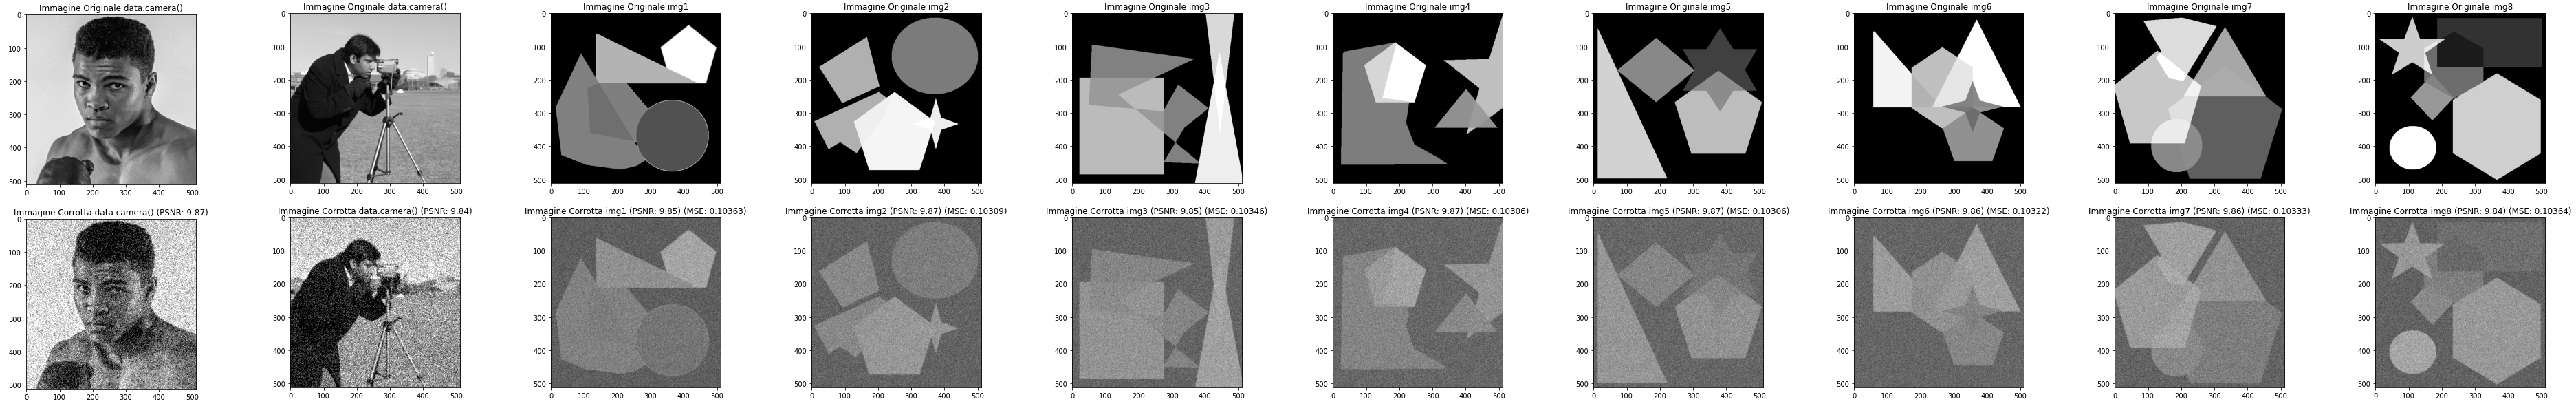
\includegraphics[width=\linewidth]{output/tabCorrotte/imgcorr10.png}\label{fig:imgcorrotte7x70.32}
    \end{minipage}
    \begin{minipage}[h]{0.55\textwidth}
        \centering
        \resizebox{1\textwidth}{!}{%
        \begin{tabular}{|l c c c c r|}
            \hline
            \rowcolor{lightbblue}\multicolumn{1}{|c}{\textbf{Nome Img}} & \multicolumn{1}{|c}{\textbf{DimKer}} & \multicolumn{1}{|c}{\textbf{Sigma}} & \multicolumn{1}{|c}{\textbf{Noise Dev}} & \multicolumn{1}{|c}{\textbf{PSNR}} & \multicolumn{1}{|c|}{\textbf{MSE}} \\ \hline
                data.camera() & 7 & 1 & 0.32 & 9.85731 & 0.10334 \\
                pugile.png & 7 & 1 & 0.32 & 9.87496 & 0.102921 \\    
                img1.png & 7 & 1 & 0.32 & 9.84505 & 0.103632 \\ 
                img2.png & 7 & 1 & 0.32 & 9.86765 & 0.103094 \\
                img3.png & 7 & 1 & 0.32 & 9.85214 & 0.103463 \\
                img4.png & 7 & 1 & 0.32 & 9.86913 & 0.103059 \\
                img5.png & 7 & 1 & 0.32 & 9.869 & 0.103062 \\
                img6.png & 7 & 1 & 0.32 & 9.86252 & 0.103216 \\ 
                img7.png & 7 & 1 & 0.32 & 9.85775 & 0.10333 \\
                img8.png & 7 & 1 & 0.32 & 9.84472 & 0.10364 \\ \hline
            \end{tabular}\label{tab:tabcorrotte7x70.32}%
        }   
        
        \end{minipage}%
    \begin{minipage}[h]{0.4\textwidth}
        \centering
        \resizebox{0.9\textwidth}{!}{%
        \begin{tabular}{|l r|}
            \hline
            \rowcolor{lightbblue}\multicolumn{2}{|c|}{\textbf{Medie calcolate}} \\ \hline
            Media PSNR           & 9.868096562243034         \\
            Media MSE            & 0.10308404121278847    \\
            Dev. Std. PSNR       & 0.009739789869654458        \\
            Dev. Std. MSE        & 0.00023117252120505893     \\ \hline
            \end{tabular}
        }
    \end{minipage}
    \captionlistentry[table]{Table corrotte}
    \captionsetup{labelformat=andtable}
    \caption{Immagini corrotte con $\sigma = 1$ dimensione $7 \times 7$ e noise = 0.32}
\end{figure}

\begin{figure}[H]
    \centering
    \begin{minipage}[h]{\textwidth}
        \centering
        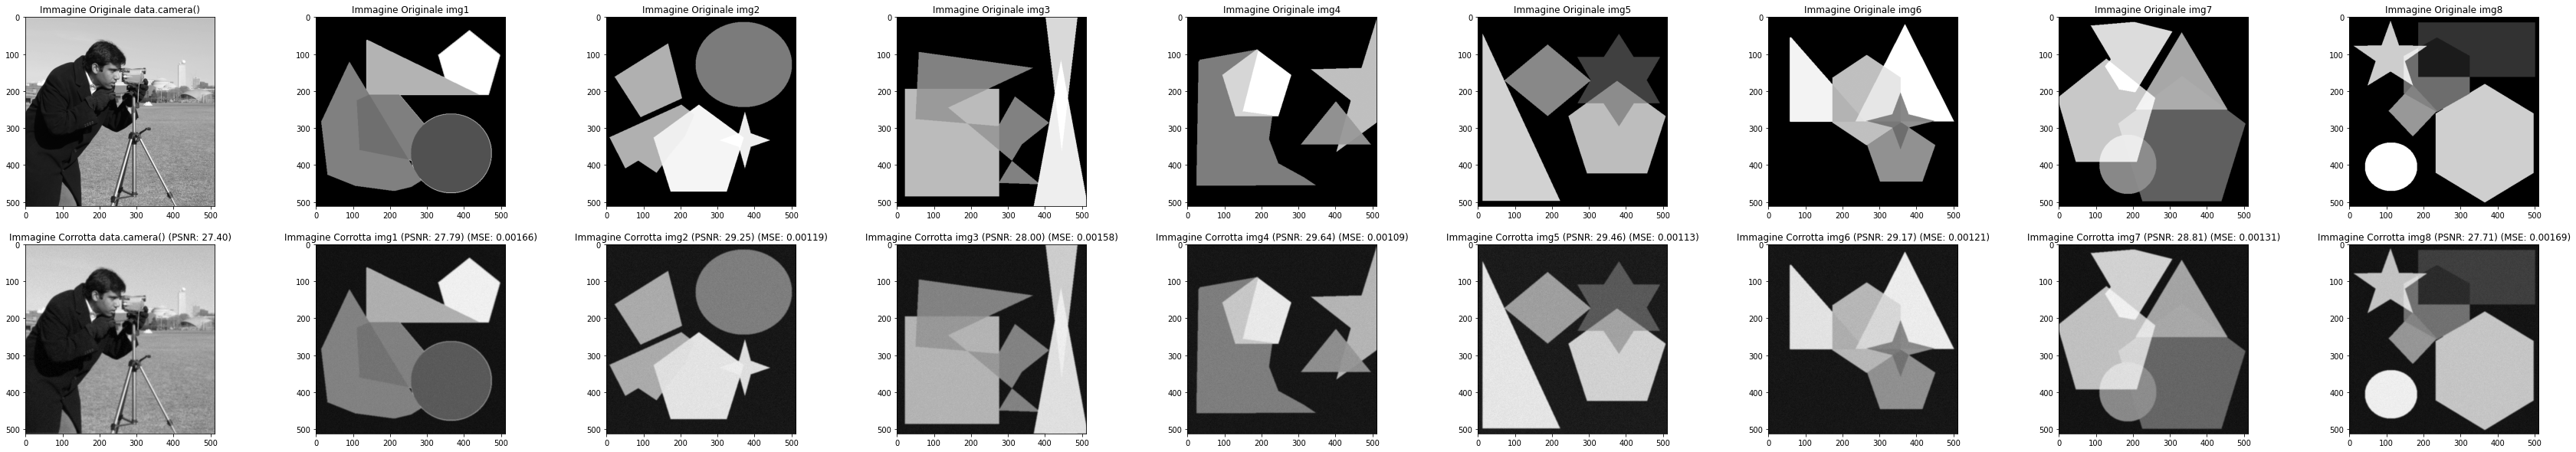
\includegraphics[width=\linewidth]{output/tabCorrotte/imgcorr11.png}\label{fig:imgcorrotte9x90.02}
    \end{minipage}
    \begin{minipage}[h]{0.55\textwidth}
        \centering
        \resizebox{1\textwidth}{!}{%
        \begin{tabular}{|l c c c c r|}
            \hline
            \rowcolor{lightbblue}\multicolumn{1}{|c}{\textbf{Nome Img}} & \multicolumn{1}{|c}{\textbf{DimKer}} & \multicolumn{1}{|c}{\textbf{Sigma}} & \multicolumn{1}{|c}{\textbf{Noise Dev}} & \multicolumn{1}{|c}{\textbf{PSNR}} & \multicolumn{1}{|c|}{\textbf{MSE}} \\ \hline
                data.camera() & 9 & 1.3 & 0.02 &  27.4138  & 0.00181392 \\
                pugile.png & 9 & 1.3 & 0.02 & 30.3576 & 0.0009209\\
                img1.png & 9 & 1.3 & 0.02 & 27.7886 & 0.00166394 \\
                img2.png & 9 & 1.3 & 0.02 & 29.2539 & 0.00118745 \\
                img3.png & 9 & 1.3 & 0.02 & 28.0014 & 0.00158437 \\
                img4.png & 9 & 1.3 & 0.02 & 29.6382 & 0.00108688 \\
                img5.png & 9 & 1.3 & 0.02 & 29.4566 & 0.00113329 \\
                img6.png & 9 & 1.3 & 0.02 & 29.1727 & 0.00120986 \\
                img7.png & 9 & 1.3 & 0.02 & 28.8132 & 0.00131424 \\
                img8.png & 9 & 1.3 & 0.02 & 27.7142 & 0.00169269 \\ \hline
        \end{tabular}\label{tab:tabcorrotte9x90.02}%
        }
    \end{minipage}%
    \begin{minipage}[h]{0.4\textwidth}
        \centering
        \resizebox{0.9\textwidth}{!}{%
        \begin{tabular}{|l r|}
            \hline
            \rowcolor{lightbblue}\multicolumn{2}{|c|}{\textbf{Medie calcolate}} \\ \hline
            Media PSNR           & 28.75660830135966        \\
            Media MSE            & 0.0013622992560759118      \\
            Dev. Std. PSNR       & 0.9328668712951993       \\
            Dev. Std. MSE        & 0.0002893379298389771   \\ \hline
            \end{tabular}
        }
    \end{minipage}
    \captionlistentry[table]{Table corrotte}
    \captionsetup{labelformat=andtable}
    \caption{Immagini corrotte con $\sigma = 1.3$ dimensione $9 \times 9$ e noise = 0.02}
\end{figure}

\begin{figure}[H]
    \centering
    \begin{minipage}[h]{\textwidth}
        \centering
        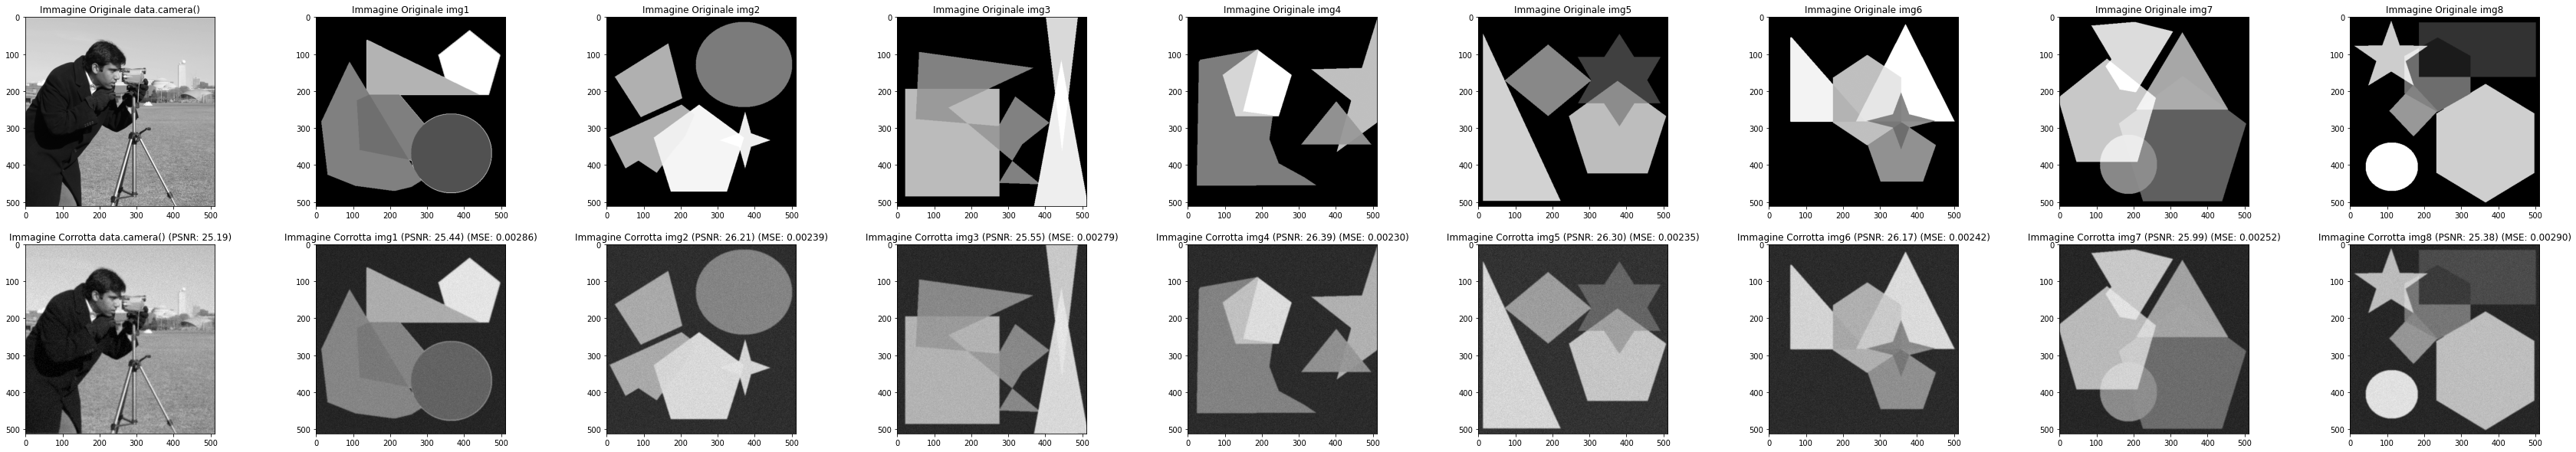
\includegraphics[width=\linewidth]{output/tabCorrotte/imgcorr12.png}\label{fig:imgcorrotte9x90.04}
    \end{minipage}
    \begin{minipage}[h]{0.55\textwidth}
        \centering
        \resizebox{1\textwidth}{!}{%
        \begin{tabular}{|l c c c c r|}
            \hline
            \rowcolor{lightbblue}\multicolumn{1}{|c}{\textbf{Nome Img}} & \multicolumn{1}{|c}{\textbf{DimKer}} & \multicolumn{1}{|c}{\textbf{Sigma}} & \multicolumn{1}{|c}{\textbf{Noise Dev}} & \multicolumn{1}{|c}{\textbf{PSNR}} & \multicolumn{1}{|c|}{\textbf{MSE}} \\ \hline
                data.camera() & 9 & 1.3 & 0.04 & 25.1912 &  0.00302606 \\   
                pugile.png & 9 & 1.3 & 0.04 & 26.7366 & 0.00212 \\
                img1.png & 9 & 1.3 & 0.04 & 25.4375 & 0.00285925 \\
                img2.png & 9 & 1.3 & 0.04 & 26.2124 & 0.00239202 \\
                img3.png & 9 & 1.3 & 0.04 & 25.5474 & 0.0027878 \\
                img4.png & 9 & 1.3 & 0.04 & 26.389 & 0.00229666 \\
                img5.png & 9 & 1.3 & 0.04 & 26.2972 & 0.00234571 \\
                img6.png & 9 & 1.3 & 0.04 & 26.1696 & 0.00241568 \\
                img7.png & 9 & 1.3 & 0.04 & 25.9907 & 0.00251728 \\
                img8.png & 9 & 1.3 & 0.04 & 25.3782 & 0.00289853 \\ \hline
            \end{tabular}\label{tab:tabcorrotte9x90.04}%
        }
        
        \end{minipage}%
    \begin{minipage}[h]{0.4\textwidth}
        \centering
        \resizebox{0.9\textwidth}{!}{%
        \begin{tabular}{|l r|}
            \hline
            \rowcolor{lightbblue}\multicolumn{2}{|c|}{\textbf{Medie calcolate}} \\ \hline
            Media PSNR           & 25.935031436703177       \\
            Media MSE            & 0.0025660139420201973     \\
            Dev. Std. PSNR       & 0.4896546967680673        \\
            Dev. Std. MSE        & 0.000289707809390377      \\ \hline
            \end{tabular}
        }
    \end{minipage}
    \captionlistentry[table]{Table corrotte}
    \captionsetup{labelformat=andtable}
    \caption{Immagini corrotte con $\sigma = 1.3$ dimensione $9 \times 9$ e noise = 0.04}
\end{figure}


\begin{figure}[H]
    \centering
    \begin{minipage}[h]{\textwidth}
        \centering
        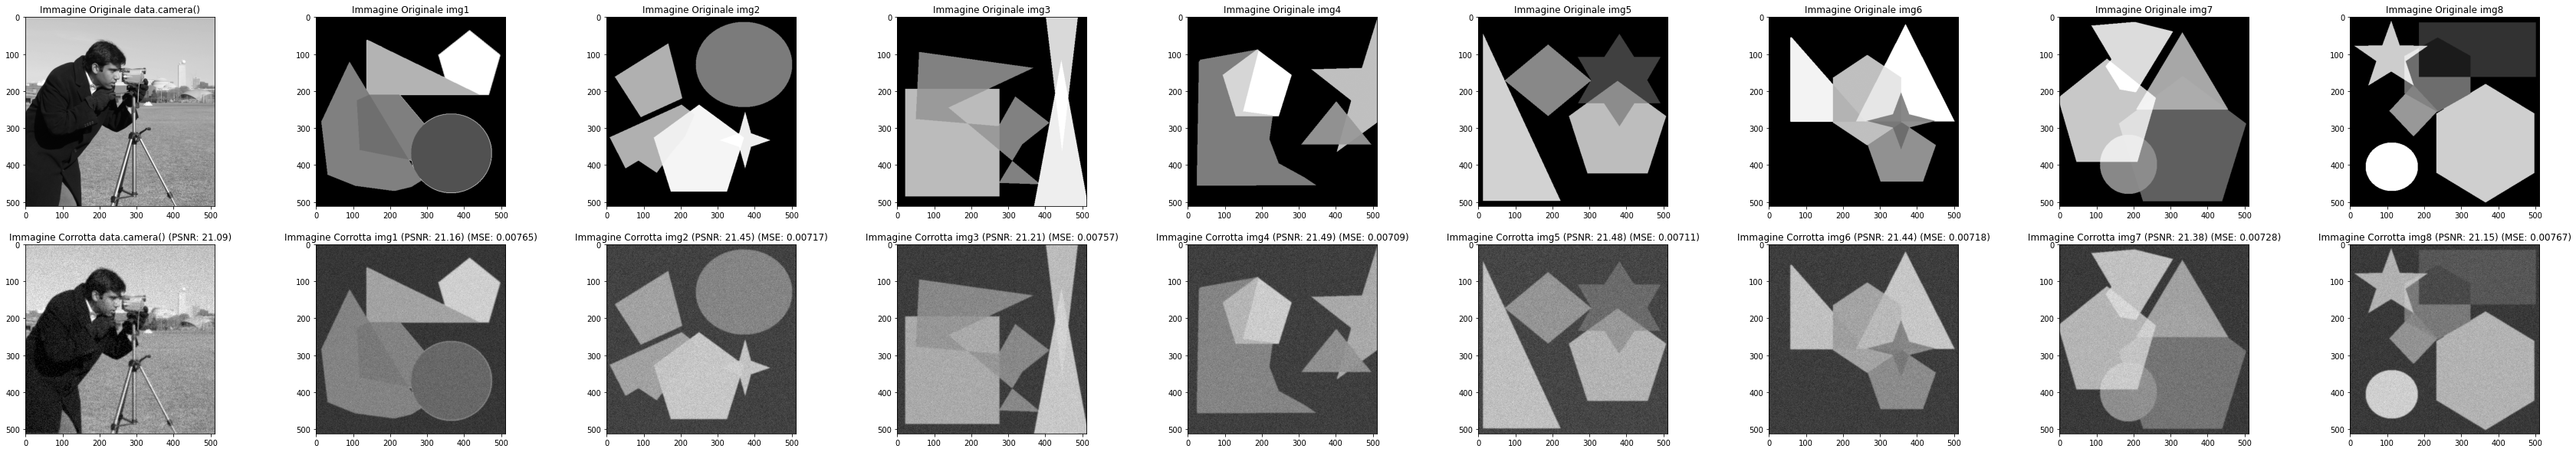
\includegraphics[width=\linewidth]{output/tabCorrotte/imgcorr13.png}\label{fig:imgcorrotte9x90.08}
    \end{minipage}
    \begin{minipage}[h]{0.55\textwidth}
        \centering
        \resizebox{1\textwidth}{!}{%
        \begin{tabular}{|l c c c c r|}
            \hline
            \rowcolor{lightbblue}\multicolumn{1}{|c}{\textbf{Nome Img}} & \multicolumn{1}{|c}{\textbf{DimKer}} & \multicolumn{1}{|c}{\textbf{Sigma}} & \multicolumn{1}{|c}{\textbf{Noise Dev}} & \multicolumn{1}{|c}{\textbf{PSNR}} & \multicolumn{1}{|c|}{\textbf{MSE}} \\ \hline
                data.camera() & 9 & 1.3 & 0.08 & 21.0692 & 0.00781774 \\    
                pugile.png & 9 & 1.3 & 0.08 & 21.6072 & 0.0069068\\
                img1.png & 9 & 1.3 & 0.08 & 21.1615 & 0.0076534 \\
                img2.png & 9 & 1.3 & 0.08 & 21.446 & 0.00716802 \\
                img3.png & 9 & 1.3 & 0.08 & 21.2099 & 0.00756858 \\
                img4.png & 9 & 1.3 & 0.08 & 21.4931 & 0.00709073 \\
                img5.png & 9 & 1.3 & 0.08 & 21.4791 & 0.0071136 \\
                img6.png & 9 & 1.3 & 0.08 & 21.436 & 0.0071845 \\
                img7.png & 9 & 1.3 & 0.08 & 21.3758 & 0.00728476 \\
                img8.png & 9 & 1.3 & 0.08 & 21.1529 & 0.00766845 \\\hline
            \end{tabular}\label{tab:tabcorrotte9x90.08}%
        }
        
        \end{minipage}%
    \begin{minipage}[h]{0.4\textwidth}
        \centering
        \resizebox{0.9\textwidth}{!}{%
        \begin{tabular}{|l r|}
            \hline
            \rowcolor{lightbblue}\multicolumn{2}{|c|}{\textbf{Medie calcolate}} \\ \hline
            Media PSNR           & 21.32346241378315          \\
            Media MSE            & 0.007378763783377743        \\
            Dev. Std. PSNR       & 0.169144238763136          \\
            Dev. Std. MSE        & 0.0002879965860764816      \\ \hline
            \end{tabular}
        }
    \end{minipage}
    \captionlistentry[table]{Table corrotte}
    \captionsetup{labelformat=andtable}
    \caption{Immagini corrotte con $\sigma = 1.3$ dimensione $9 \times 9$ e noise = 0.08}
\end{figure}

\begin{figure}[H]
    \centering
    \begin{minipage}[h]{\textwidth}
        \centering
        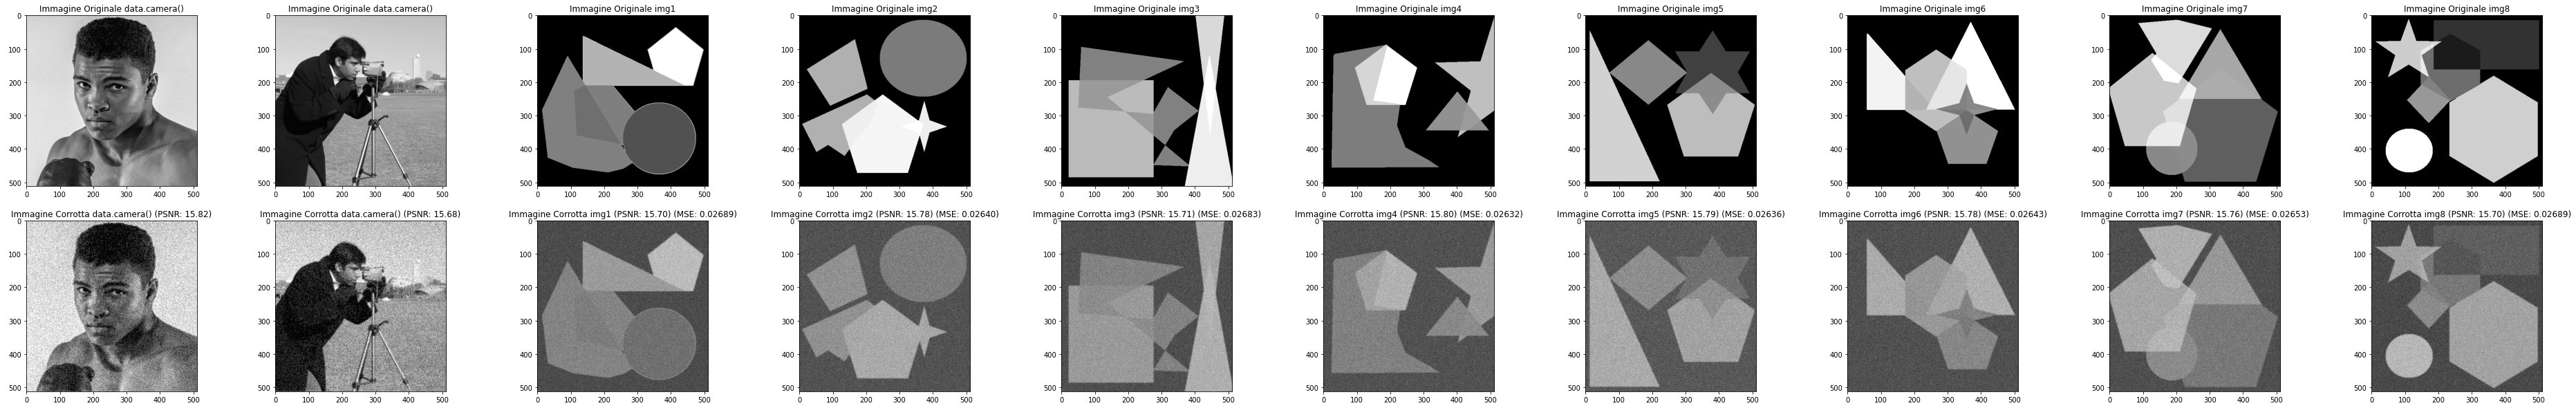
\includegraphics[width=\linewidth]{output/tabCorrotte/imgcorr14.png}\label{fig:imgcorrotte9x90.16}
    \end{minipage}
    \begin{minipage}[h]{0.55\textwidth}
        \centering
        \resizebox{1\textwidth}{!}{%
        \begin{tabular}{|l c c c c r|}
            \hline
            \rowcolor{lightbblue}\multicolumn{1}{|c}{\textbf{Nome Img}} & \multicolumn{1}{|c}{\textbf{DimKer}} & \multicolumn{1}{|c}{\textbf{Sigma}} & \multicolumn{1}{|c}{\textbf{Noise Dev}} & \multicolumn{1}{|c}{\textbf{PSNR}} & \multicolumn{1}{|c|}{\textbf{MSE}} \\ \hline
                data.camera() & 9 & 1.3 & 0.16 & 15.6736 & 0.0270796 \\  
                pugile.png & 9 & 1.3 & 0.16 & 15.8334 & 0.0261013\\
                img1.png & 9 & 1.3 & 0.16 & 15.7044 & 0.026888 \\
                img2.png & 9 & 1.3 & 0.16 & 15.7843 & 0.0263979 \\
                img3.png & 9 & 1.3 & 0.16 & 15.7146 & 0.0268251 \\
                img4.png & 9 & 1.3 & 0.16 & 15.7966 & 0.026323 \\
                img5.png & 9 & 1.3 & 0.16 & 15.7911 & 0.0263568 \\
                img6.png & 9 & 1.3 & 0.16 & 15.7794 & 0.0264277 \\
                img7.png & 9 & 1.3 & 0.16 & 15.7632 & 0.0265265 \\
                img8.png & 9 & 1.3 & 0.16 & 15.7044 & 0.0268884 \\\hline
            \end{tabular}\label{tab:tabcorrotte9x90.16}%
        }
        
        \end{minipage}%
    \begin{minipage}[h]{0.4\textwidth}
        \centering
        \resizebox{0.9\textwidth}{!}{%
        \begin{tabular}{|l r|}
            \hline
            \rowcolor{lightbblue}\multicolumn{2}{|c|}{\textbf{Medie calcolate}} \\ \hline
            Media PSNR           & 15.752586448516155       \\
            Media MSE            & 0.026593095526593946      \\
            Dev. Std. PSNR       & 0.04888788575026526        \\
            Dev. Std. MSE        & 0.00029971901539735954    \\ \hline
            \end{tabular}
        }
    \end{minipage}
    \captionlistentry[table]{Table corrotte}
    \captionsetup{labelformat=andtable}
    \caption{Immagini corrotte con $\sigma = 1.3$ dimensione $9 \times 9$ e noise = 0.16}
\end{figure}



\begin{figure}[H]
    \centering
    \begin{minipage}[h]{\textwidth}
        \centering
        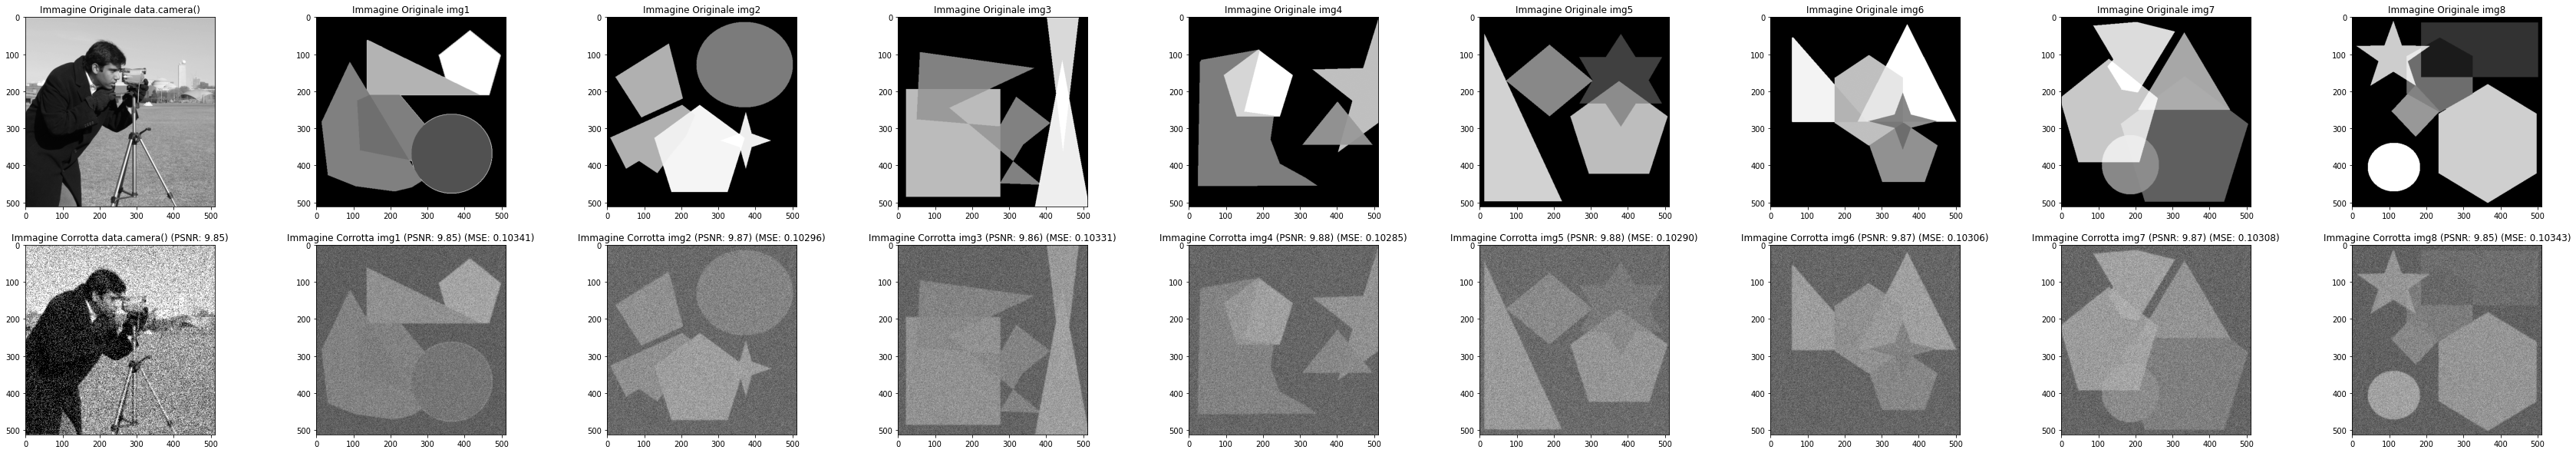
\includegraphics[width=\linewidth]{output/tabCorrotte/imgcorr15.png}\label{fig:imgcorrotte9x90.32}
    \end{minipage}
    \begin{minipage}[h]{0.55\textwidth}
        \centering
        \resizebox{1\textwidth}{!}{%
        \begin{tabular}{|l c c c c r|}
            \hline
            \rowcolor{lightbblue}\multicolumn{1}{|c}{\textbf{Nome Img}} & \multicolumn{1}{|c}{\textbf{DimKer}} & \multicolumn{1}{|c}{\textbf{Sigma}} & \multicolumn{1}{|c}{\textbf{Noise Dev}} & \multicolumn{1}{|c}{\textbf{PSNR}} & \multicolumn{1}{|c|}{\textbf{MSE}} \\ \hline
                data.camera() & 9 & 1.3 & 0.32 & 9.82272 & 0.104167 \\   
                pugile.png & 9 & 1.3 & 0.32 & 9.88385 & 0.10271 \\
                img1.png & 9 & 1.3 & 0.32 & 9.85454 & 0.103406 \\
                img2.png & 9 & 1.3 & 0.32 & 9.87346 & 0.102957 \\
                img3.png & 9 & 1.3 & 0.32 & 9.85875 & 0.103306 \\
                img4.png & 9 & 1.3 & 0.32 & 9.87778 & 0.102854 \\
                img5.png & 9 & 1.3 & 0.32 & 9.87599 & 0.102897 \\
                img6.png & 9 & 1.3 & 0.32 & 9.86911 & 0.10306 \\ 
                img7.png & 9 & 1.3 & 0.32 & 9.8681 & 0.103084 \\ 
                img8.png & 9 & 1.3 & 0.32 & 9.85336 & 0.103434 \\\hline
            \end{tabular}\label{tab:tabcorrotte9x90.32}%
        }
        
        \end{minipage}%
    \begin{minipage}[h]{0.4\textwidth}
        \centering
        \resizebox{0.9\textwidth}{!}{%
        \begin{tabular}{|l r|}
            \hline
            \rowcolor{lightbblue}\multicolumn{2}{|c|}{\textbf{Medie calcolate}} \\ \hline
            Media PSNR           & 9.842576581447004           \\
            Media MSE            & 0.10369173965451903     \\
            Dev. Std. PSNR       & 0.012567871393636715        \\
            Dev. Std. MSE        & 0.0003001770981803593     \\ \hline
            \end{tabular}
        }
    \end{minipage}
    \captionlistentry[table]{Table corrotte}
    \captionsetup{labelformat=andtable}
    \caption{Immagini corrotte con $\sigma = 1.3$ dimensione $9 \times 9$ e noise = 0.32}
\end{figure}

\begin{figure}[H]
    \centering
    \begin{minipage}[h]{\textwidth}
        \centering
        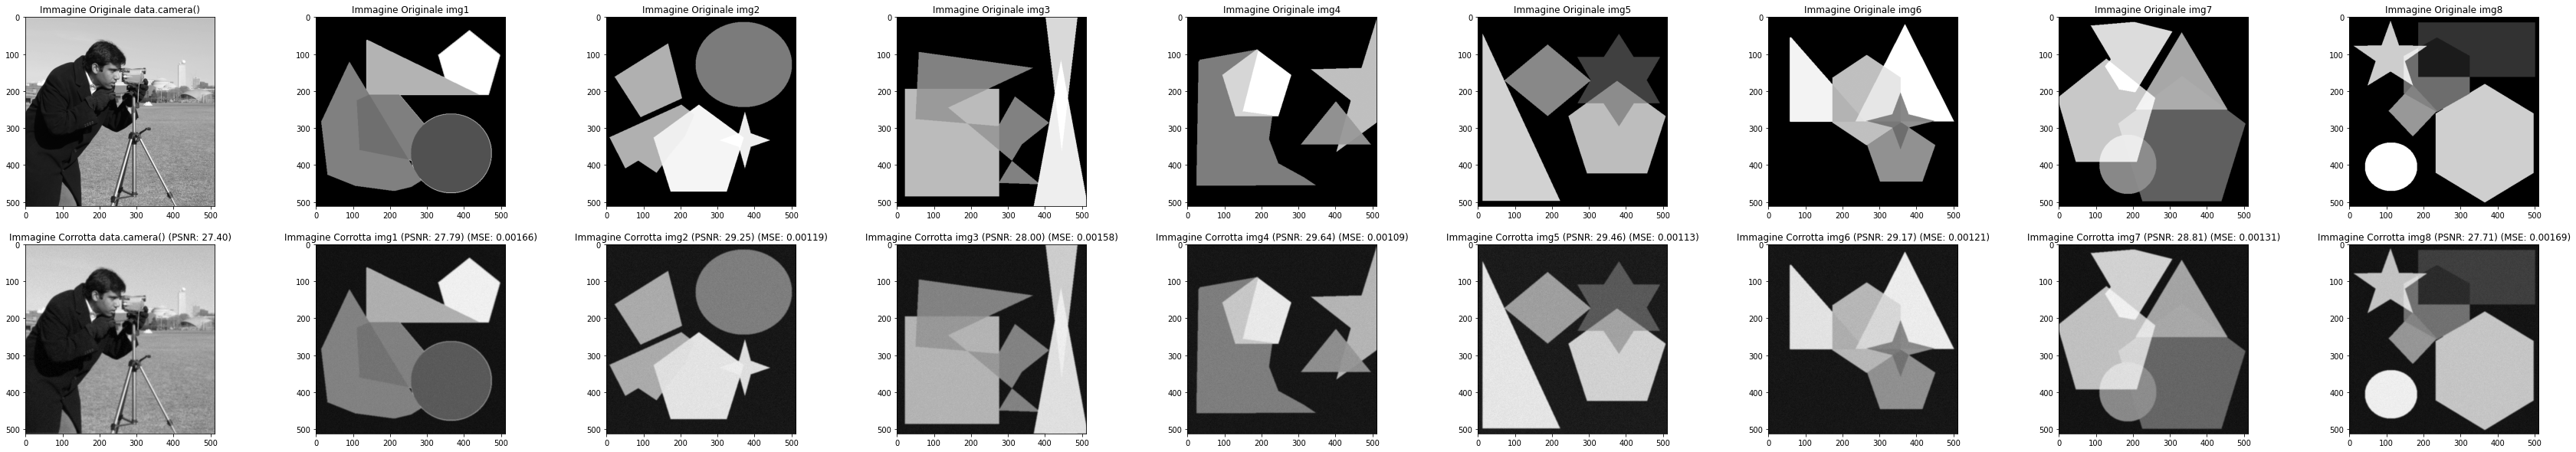
\includegraphics[width=\linewidth]{output/tabCorrotte/imgcorr11.png}\label{fig:imgcorrotteGEN}
    \end{minipage}
    \begin{minipage}[h]{0.4\textwidth}
        \centering
        \resizebox{0.9\textwidth}{!}{%
        \begin{tabular}{|l r|}
            \hline
            \rowcolor{lightbblue}\multicolumn{2}{|c|}{\textbf{Istanza del Problema}} \\ \hline
            Media PSNR           & 28.75660830135966        \\
            Media MSE            & 0.0013622992560759118      \\
            Dev. Std. PSNR       & 0.9328668712951993       \\
            Dev. Std. MSE        & 0.0002893379298389771   \\ \hline
            \end{tabular}
        }
    \end{minipage}
    \captionlistentry[table]{Table corrotte}
    \captionsetup{labelformat=andtable}
    \caption{Immagini corrotte con noise = 0.02, $\sigma = 1.3$ dimensione $9 \times 9$}
\end{figure}

Notiamo che tutte le immagini all'aumentare del valore rumore "\verb|noise|" peggiorano 
qualitativamente: 
con $\sigma = 0.5$ e noise 0.02 abbiamo per esempio un valore medio del PSNR in 
media vicino a 30, invece aumentando il noise a 0.32 scende addirittura attorno a 9, con 
immagini che tendono a risultare molto sfocate e disturbate dal rumore guassiano. 
Inoltre quando il rumore è alto, le deviazioni standard tendono a diminuire: 
infatti i valori di PSNR e MSE sono pressocchè uguali tra di loro, quasi come se fossero stati pareggiati (o livellati). 

All'aumentare delle dimensioni del Kernel ($\sigma = 1$ e dimensioni $7 \times 7$) notiamo che partendo 
da un rumore pari a 0.02 abbiamo un PSNR in media leggermente inferiore rispetto alla precedente 
dimensione del Kernel.
La cosa si ripete quando si passa a $\sigma = 1.3$.
I valori di PSNR delle rispettive immagini decrescono 
rispetto ai valori ottenuti dalle precedenti dimensioni del Kernel con lo stesso valore noise fissato.
    \subsection{Osservazioni}
Osserviamo il risultato su un'immagine scelta casualmente del set creato e sulle due immagini aggiuntive.
%! l'elemento principale e' il rumore + mettere confronti

Ricordiamo che più è alto il valore del PSNR maggiore sarà la vicinanza dell'immagine corrotta rispetto alla versione originale. 

\subsubsection{Analisi immagine geometrica}
Analizziamo l'immagine img8.png al variare del valore $\sigma$:

\begin{figure}[H]
    \centering
    \begin{subfigure}{0.6\textwidth}
        \centering
        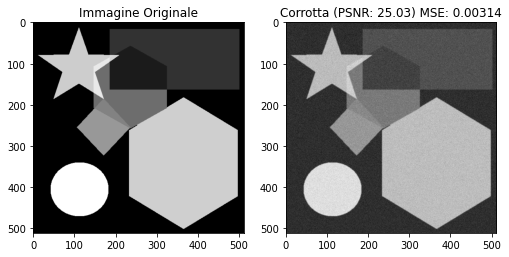
\includegraphics[width=\textwidth]{imgRel/img8corrotto/img8corrotta5x5.png}
        \caption{Img8 corrotta con $\sigma = 0.5$ dimensione $5 \times 5$}
        \label{fig:8corrotto5}
    \end{subfigure}
    \begin{subfigure}{0.6\textwidth}
        \centering
        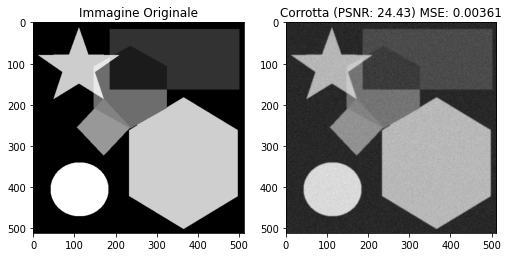
\includegraphics[width=\textwidth]{imgRel/img8corrotto/img8corrotta7x7.png}
        \caption{Img8 corrotta con $\sigma = 1$ dimensione $7\times 7$}
        \label{fig:8corrotto7}
    \end{subfigure}
    \begin{subfigure}{0.6\textwidth}
        \centering
        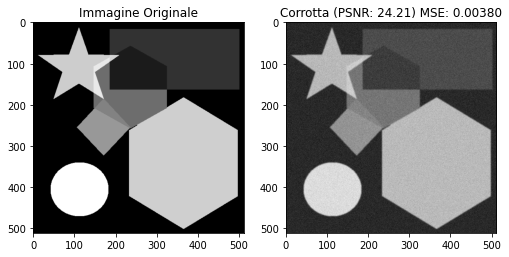
\includegraphics[width=\textwidth]{imgRel/img8corrotto/img8corrotta9x9.png}
        \caption{Img8 corrotta con $\sigma = 1.3$ dimensione $9 \times 9$}
        \label{fig:8corrotto9}
    \end{subfigure}
    \caption{Immagine geometrica corrotta al variare di $\sigma$}
    \label{fig:8corrotto}
\end{figure}
Le figure di sinistra rappresentano l'immagine originale, invece a destra sono riportate le immagini corrotte con i rispettivi valori di PSNR. 
Notiamo che all'aumentare delle dimensioni di sigma il valore di PSNR diminuisce che denota un peggioramento della qualità dell'immagine, 
infatti le immagini subiscono un'appiattimento dell'intensità della scala dei colori e i contorni delle varie figure geometriche perdono di fermezza. 
%! da finire

\subsubsection{Analisi immagini fotografiche}
\begin{figure}[H]
    \centering
    \begin{subfigure}{0.67\textwidth}
        \centering
        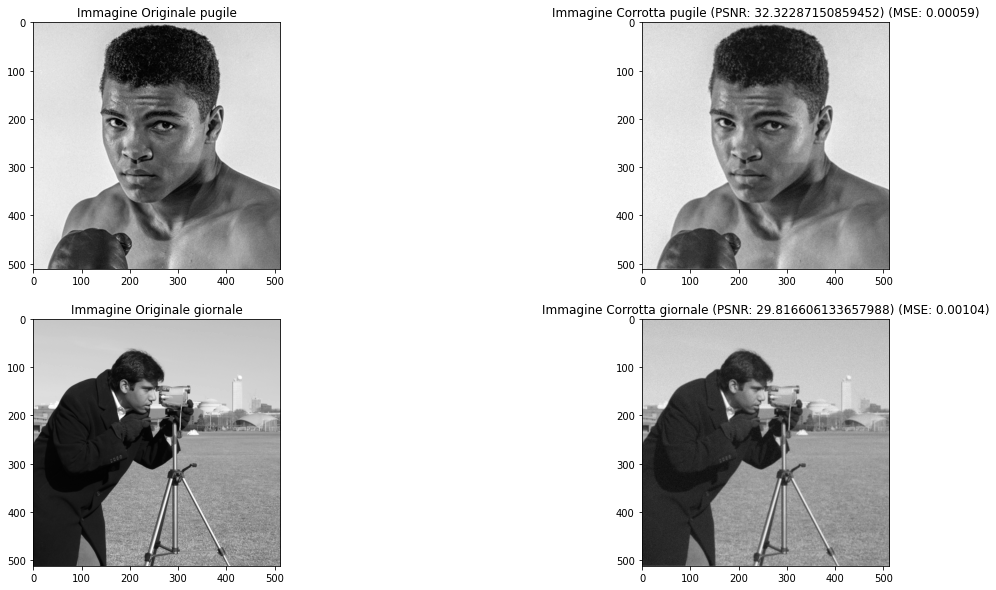
\includegraphics[width=\textwidth]{confrontiPuntoUno/5-0.5-0.02.png}
        \caption{immagini corrotte con $\sigma = 0.5$ dimensione $5 \times 5$}
        \label{fig:fotogrCorrotte5x5}
    \end{subfigure}
    \begin{subfigure}{0.67\textwidth}
        \centering
        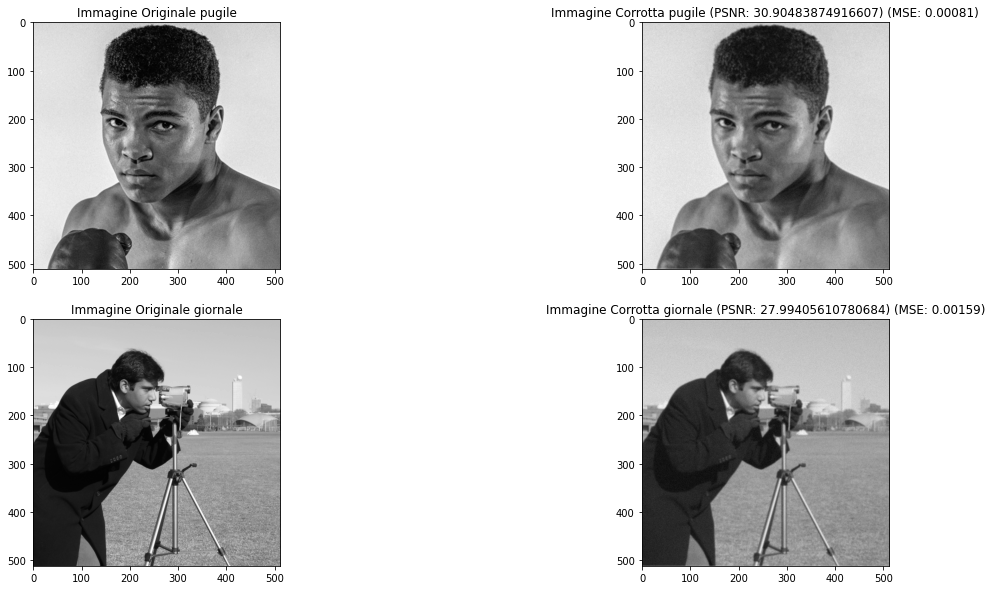
\includegraphics[width=\textwidth]{confrontiPuntoUno/7-1-0.02.png}
        \caption{immagini corrotte con $\sigma = 1$ dimensione $7 \times 7$}
        \label{fig:fotogrCorrotte7x7}
    \end{subfigure}
    \begin{subfigure}{0.67\textwidth}
        \centering
        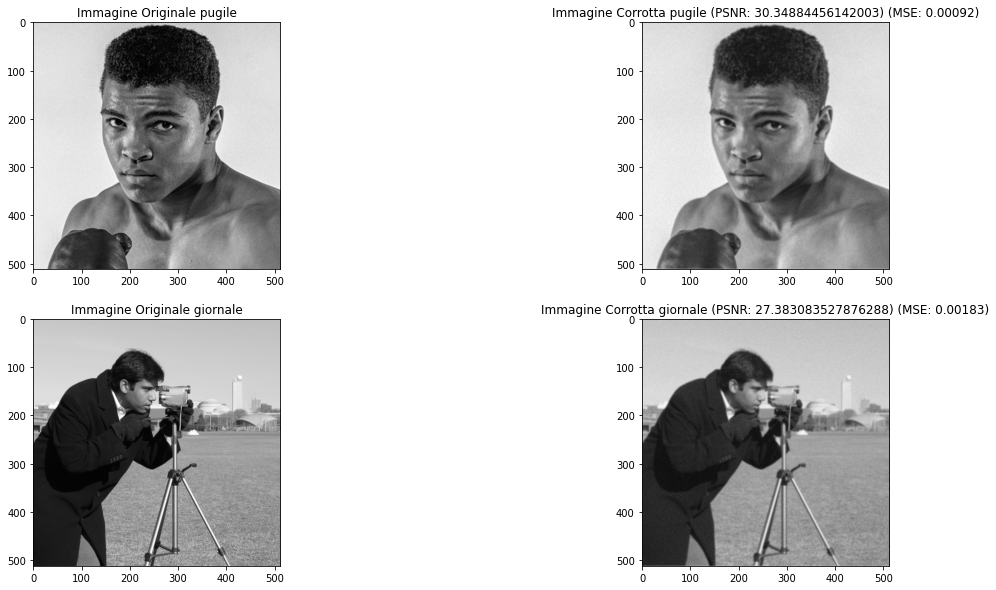
\includegraphics[width=\textwidth]{confrontiPuntoUno/9-1.3-0.02.png}
        \caption{immagini corrotte con $\sigma = 1.3$ dimensione $9 \times 9$}
        \label{fig:fotogrCorrotte9x9}
    \end{subfigure}
    \caption{Immagine fotografica corrotta al variare di $\sigma$}
    \label{fig:fotogrCorrotte}
\end{figure}

Si nota un'altra volta che all'aumentare delle dimensioni di $\sigma$ diminuisce il PSNR e l'immagine perde di 
incisività, le versioni corrotte benché risultino visivamente peggiori, si riesce ancora a ben distinguere il 
soggetto in primo piano, anche se sfocato, in tutte le immagini. 

\section{Ricostruzione di un immagine rispetto una versione corrotta}
Una possibile ricostruzione dell'immagine originale $x$ partendo dall'immagine corrotta $b$ è la soluzione naive data dal minimo del seguente problema di ottimizzazione:
\[x^* = \arg\min_x \frac{1}{2} ||Ax - b||_2^2\]

Nell'analisi delle immagini ricostruite useremo $\sigma=1$ dimensione $7\times 7$ come valore standard.
%! immagine grafico  mg vs mgc

Abbiamo mostrato questi due grafici sovrastanti perché si evince che all'aumentare del numero delle 
iterazioni l'immagine ricavata si allontana dalla sua versione originale poiché è presente una deviazione. 


    \subsection{Metodo del Gradiente Coniugato (naive)}
Il metodo del gradiente coniugato è un algoritmo per la risoluzione numerica di un sistema lineare la cui matrice sia simmetrica e definita positiva
 e consente di risolvere il sistema in un numero di iterazioni che è al massimo $n$.

La funzione $f$ da minimizzare è data dalla formula
  $f(x) = \frac{1}{2} ||Ax - b||_2^2 $, il cui gradiente $\nabla f$ è dato da
$\nabla f(x) = A^TAx - A^Tb  $.

Utilizzando il metodo del gradiente coniugato implementato dalla funzione \code{minimize}
 abbiamo calcolato la soluzione naive.

\begin{figure}[H]
  \centering
  \begin{subfigure}{0.9\textwidth}
    \centering
    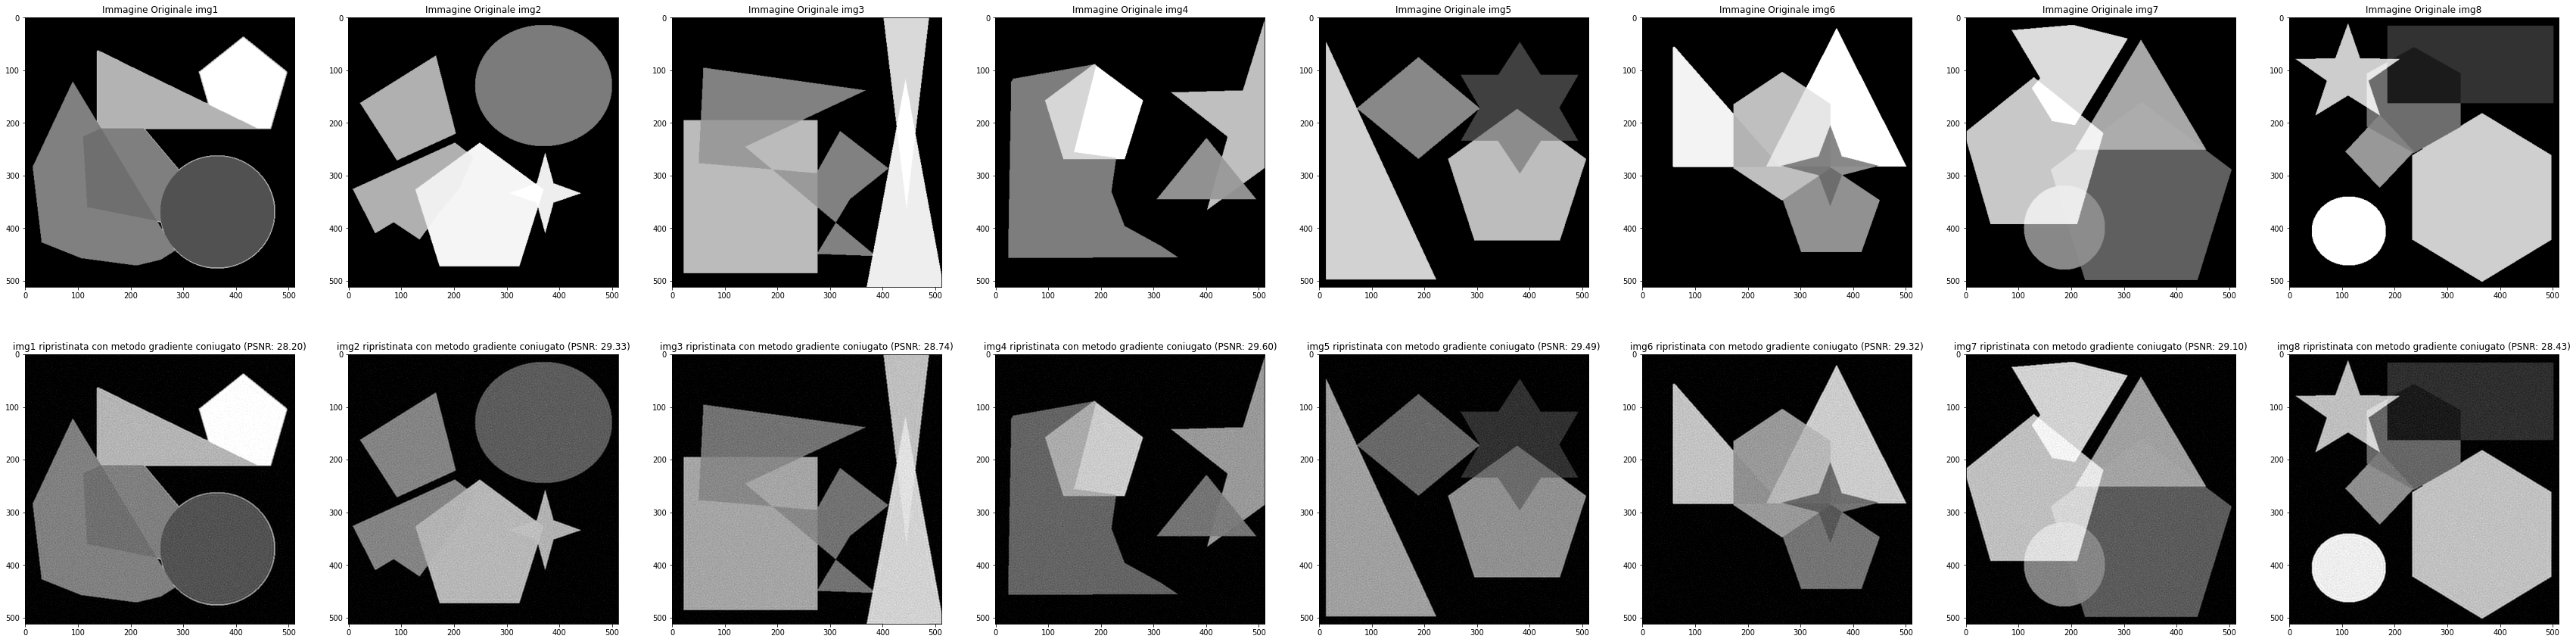
\includegraphics[width=0.9\textwidth]{imgRel/datasetconiugato.png}
    \caption{Immagini geometriche ripristinate con il Metodo del Gradiente Coniugato}
    \label{fig:geomripristinate}
  \end{subfigure}

  \begin{subfigure}{0.5\textwidth}
    \centering
    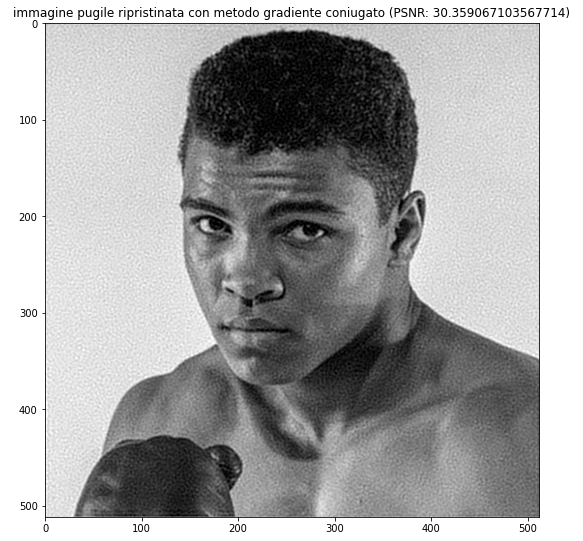
\includegraphics[width=\textwidth]{imgRel/pugilemgc.png}
    \caption{Immagine fotografica ripristinata con il Metodo del Gradiente Coniugato}
  \end{subfigure}\hfill
  \begin{subfigure}{0.5\textwidth}
    
\includegraphics[width=\textwidth]{imgRel/giornalemgc.png}
    \caption{Immagine con testo ripristinata con il Metodo del Gradiente Coniugato}
  \end{subfigure}
  \caption{Immagini analizzate ripristinate con il Metodo del Gradiente Coniugato}

  \centering
    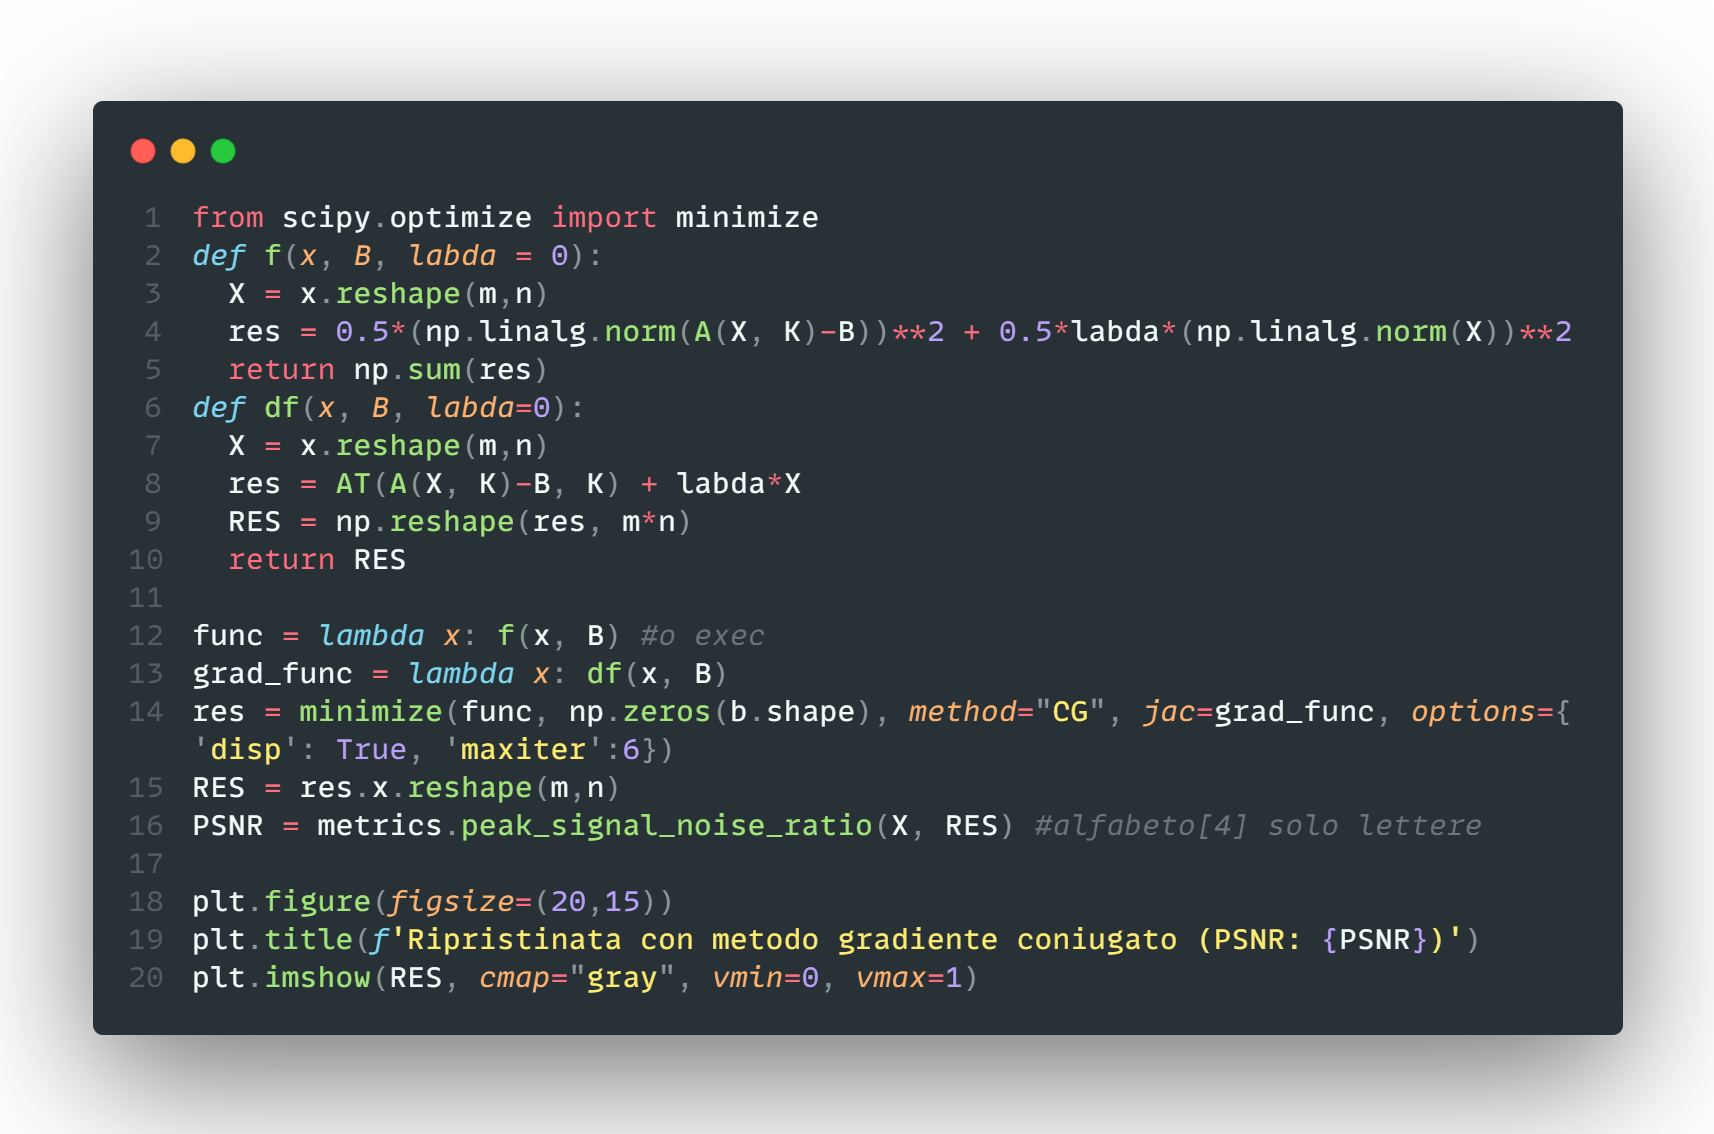
\includegraphics[width=0.6\textwidth]{imgCode/metGradCon.png}
    \caption{Codice Metodo del Gradiente Coniugato applicato ad una singola immagine}
    \label{fig:codeMGC}
\end{figure}


    \subsection{Metodo del Gradiente}
Il metodo del gradiente è un algoritmo che calcola il vettore di minimo globale, ovvero:
Un vettore $x^{\ast}$ è un punto di minimo globale di $f(x)$ se $f(x^{\ast}) \leq f(x) \forall x \in R^n$.

Analogamente, un vettore $x^{\ast}$ è un punto di minimo globale in senso stretto di $f(x)$ 
se $f(x^{\ast}) < f(x) \forall x \in R+n \and x \neq x^{\ast}$.

\begin{figure}[H]
    \centering
    \begin{subfigure}{0.9\textwidth}
        \centering
    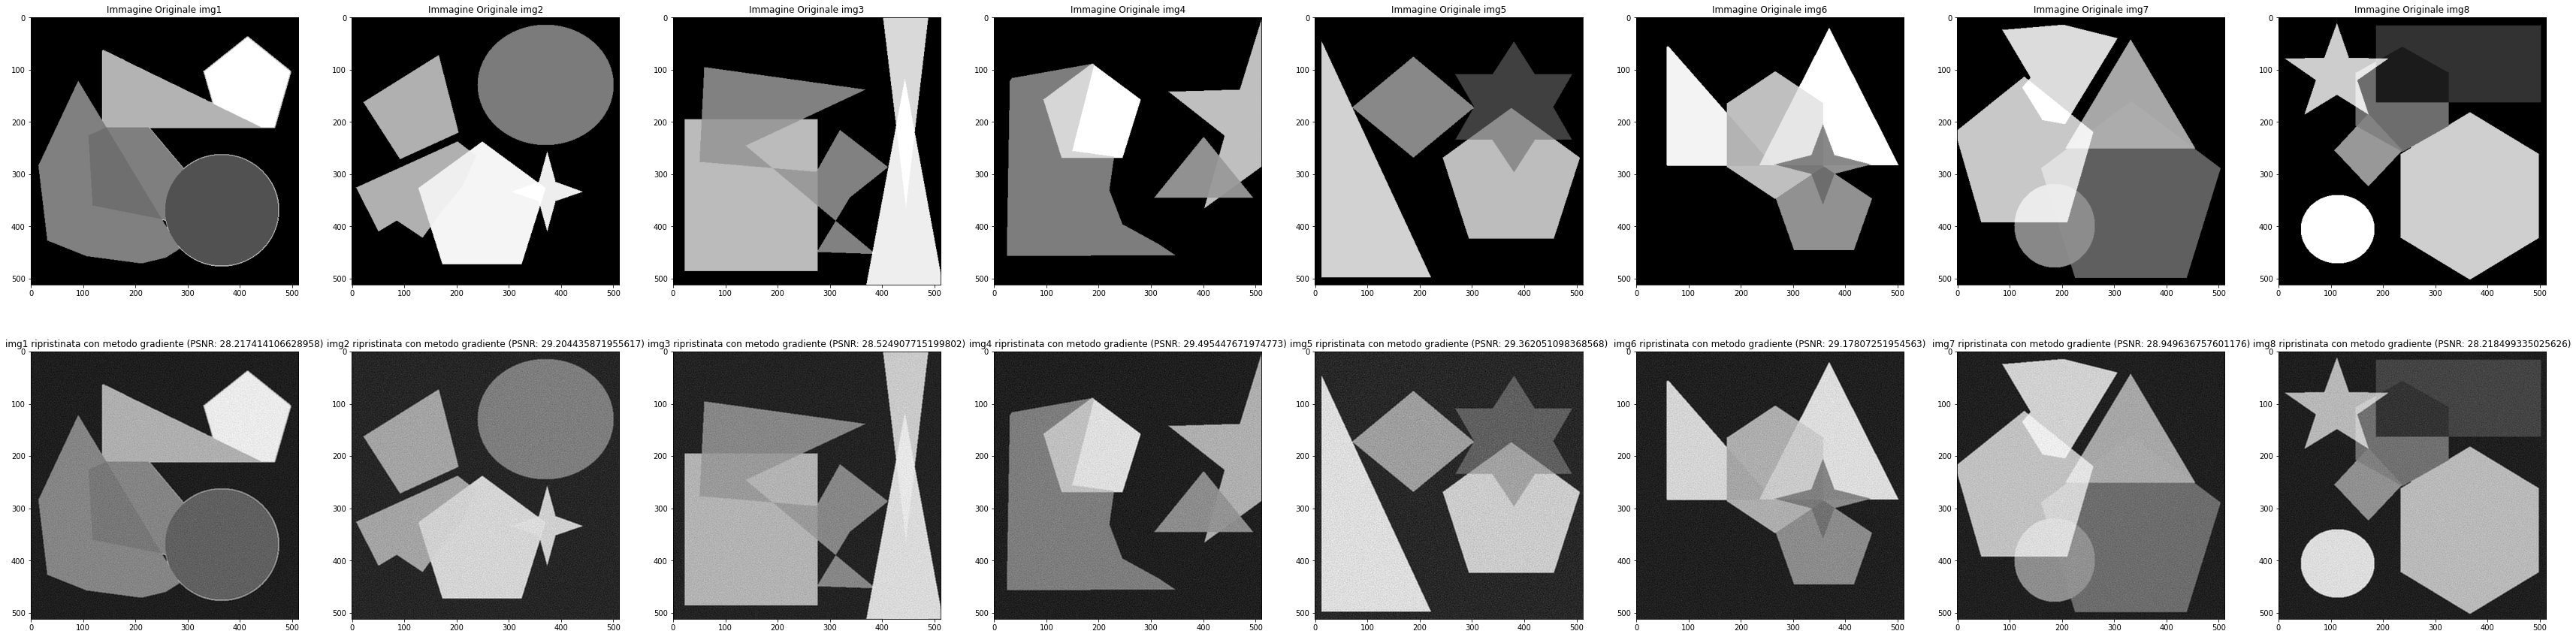
\includegraphics[width=0.7\textwidth]{imgRel/datasetgradiente.png}
    \caption{Immagini geometriche ripristinate}
    \label{fig:geomgradiente}
    \end{subfigure}

    \begin{subfigure}{0.5\textwidth}
        \centering
    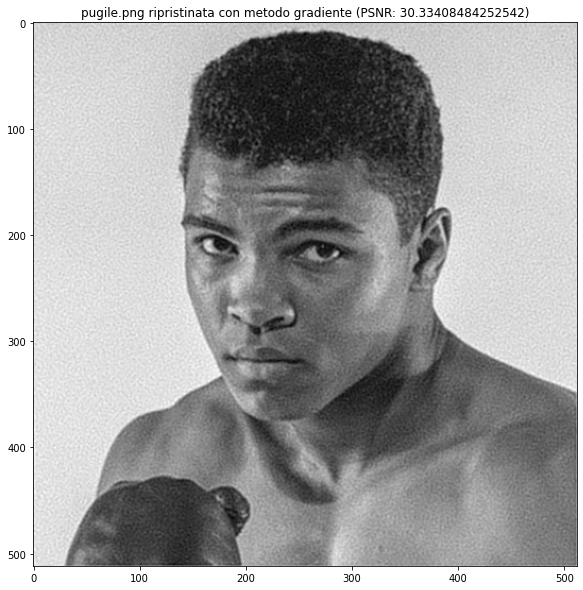
\includegraphics[width=0.6\linewidth]{imgRel/fotogrmg.png}
    \caption{Immagine fotografica ripristinata}
    \label{fig:pugilegradiente}
    \end{subfigure}%
    \begin{subfigure}{0.5\textwidth}\centering
        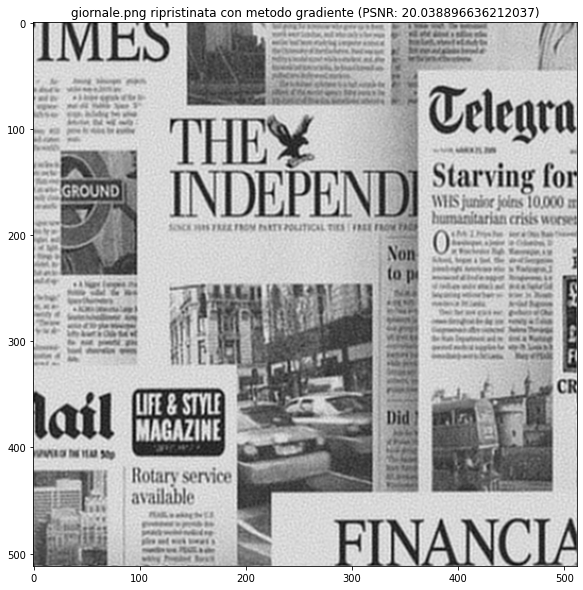
\includegraphics[width=0.6\linewidth]{imgRel/giornalemg.png}
        \caption{Immagine con testo ripristinata}
    \end{subfigure}
\caption{Immagini analizzate ripristinate con il Metodo del Gradiente}
\end{figure}
\begin{figure}[H]
    \centering
    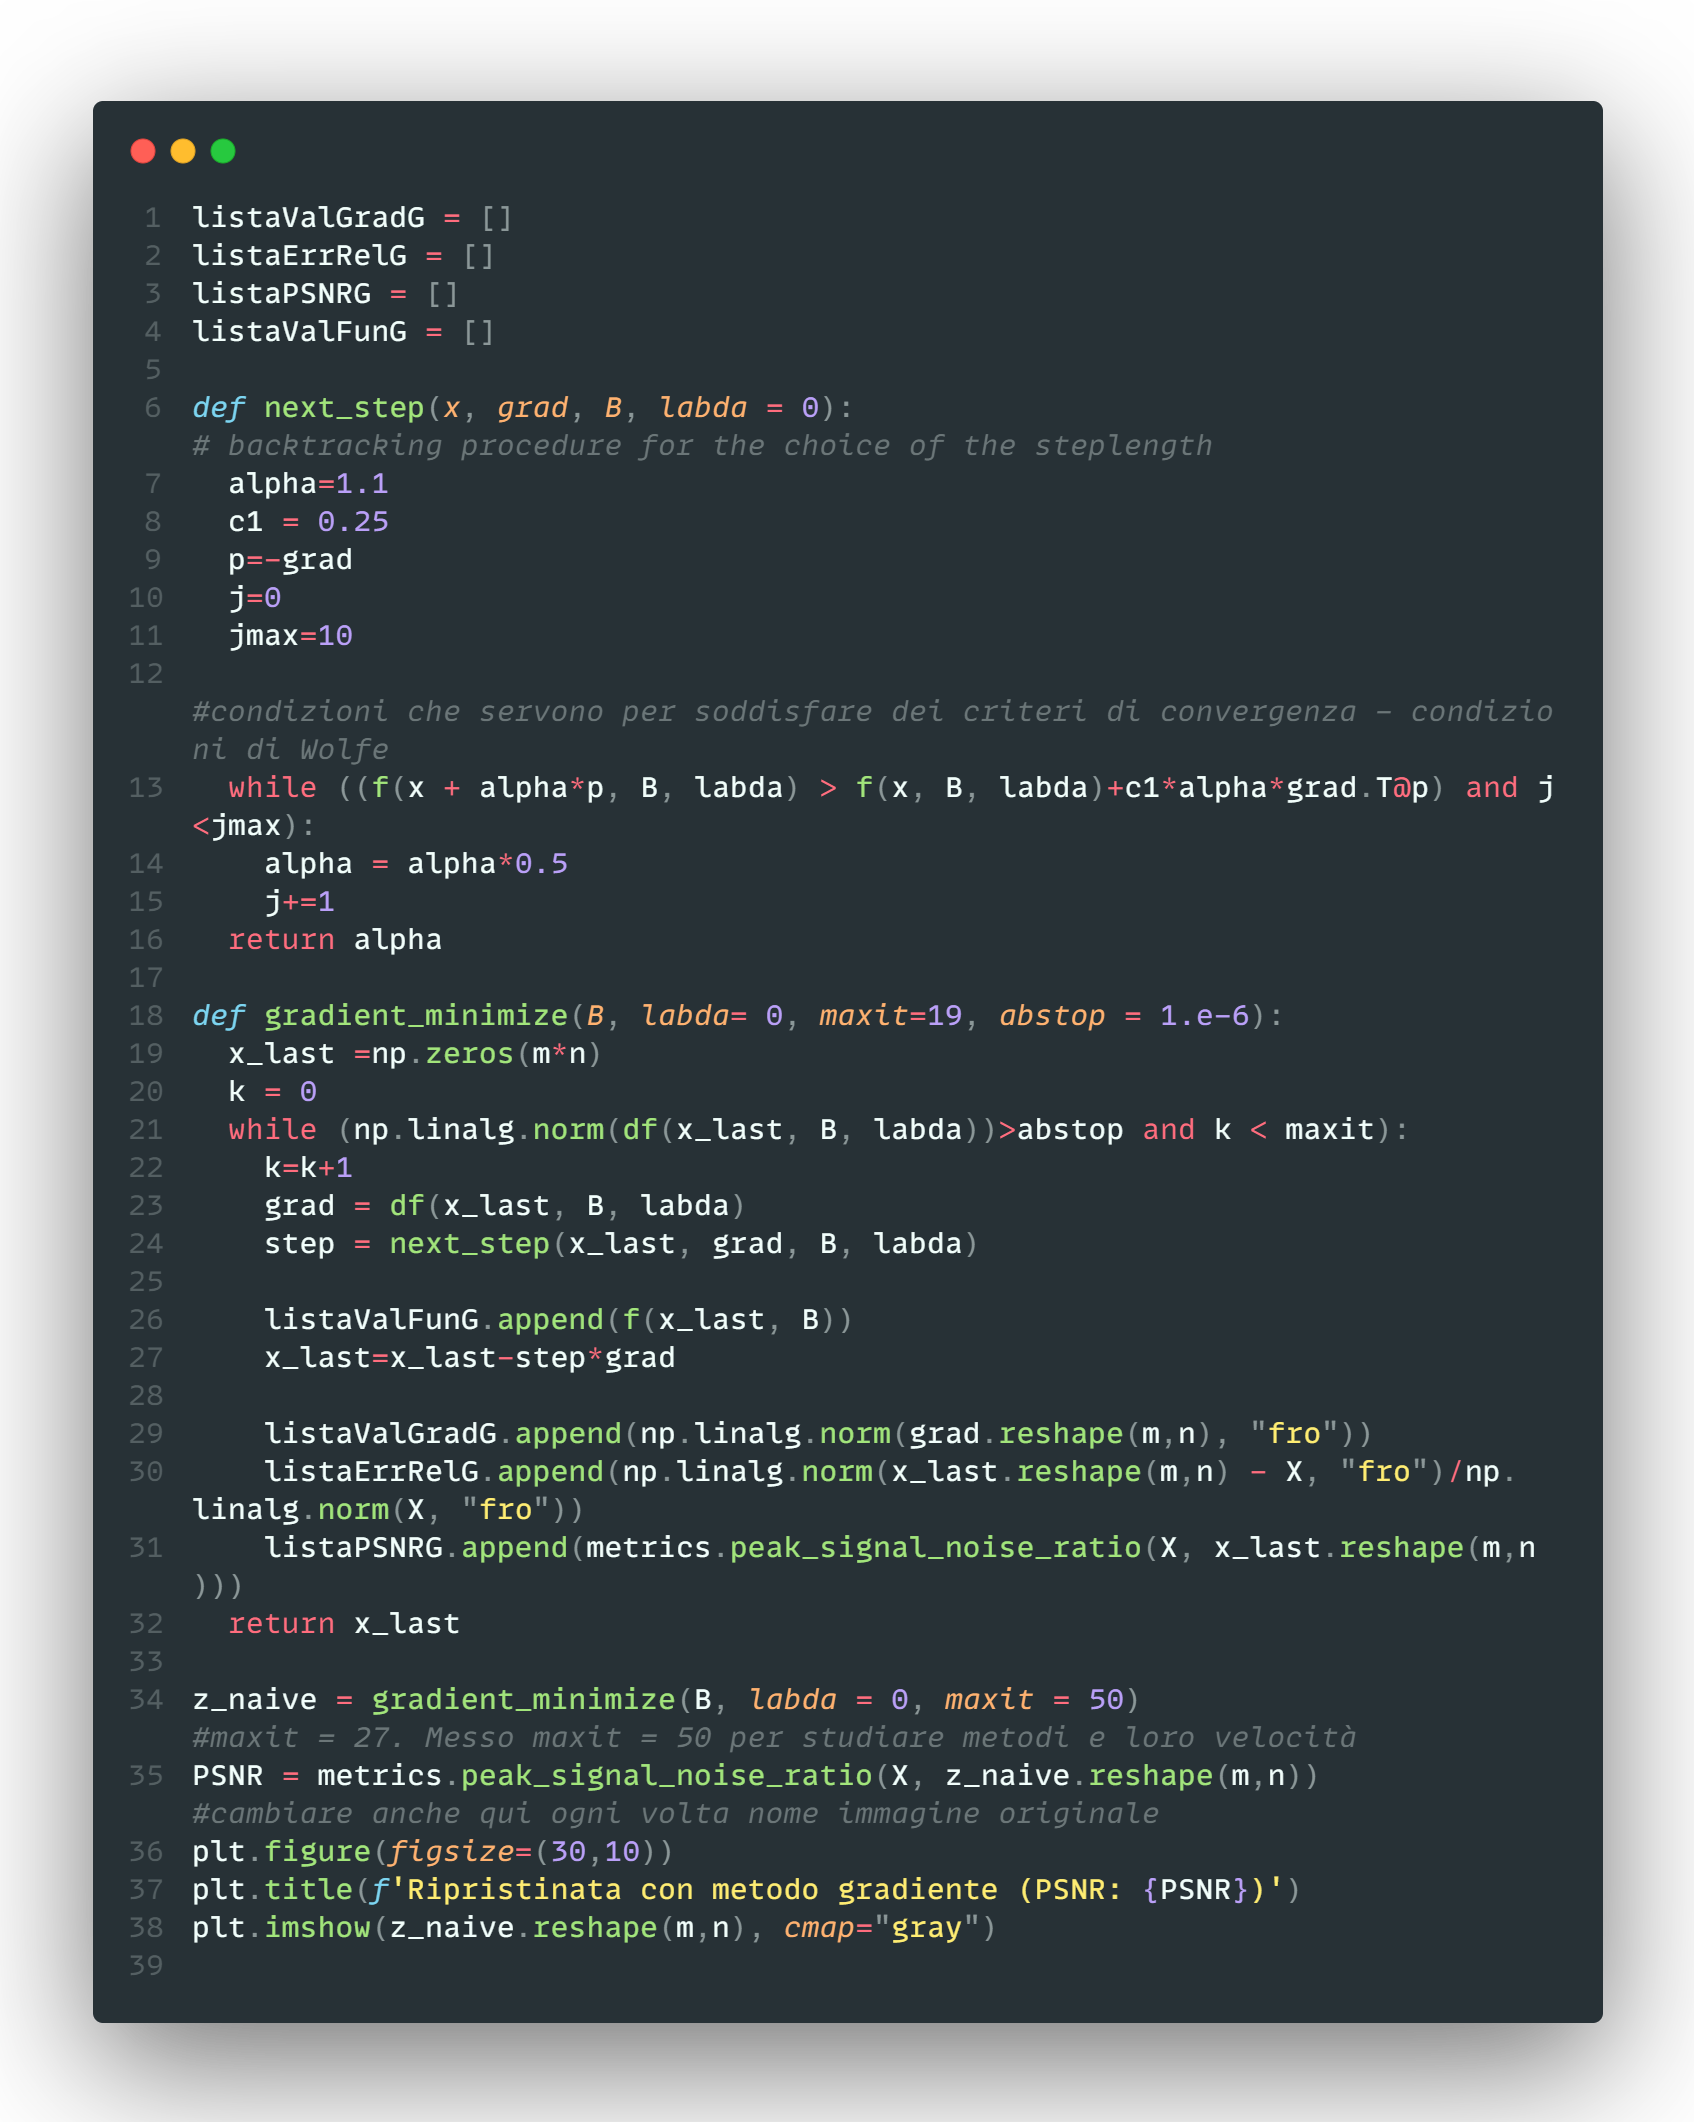
\includegraphics[width=0.7\textwidth]{imgCode/metGrad.png}
    \caption{Codice Metodo del gradiente applicato ad una singola immagine}
\end{figure}



\end{document}